\documentclass[12pt, a4paper]{article}

% --- Encoding & Language ---
\usepackage{fontspec}
\usepackage{polyglossia}
\setmainlanguage{vietnamese}
\setotherlanguage{english}
\setmainfont{Times New Roman}
\setmonofont{Courier New}

% --- Layout ---
\usepackage[top=2.5cm, bottom=2.5cm, left=3cm, right=2.5cm]{geometry}
\usepackage{setspace}
\onehalfspacing

% --- Math ---
\usepackage{amsmath, amssymb, amsthm}

% --- Figures & Tables ---
\usepackage{graphicx}
\usepackage{float}
\usepackage{booktabs}
\usepackage{tabularx}
\usepackage{multirow}
\usepackage{caption}
\usepackage{subcaption}
\captionsetup{font=small, labelfont=bf}

% --- Code listings (minimal use) ---
\usepackage{listings}
\usepackage{xcolor}
\definecolor{codebg}{HTML}{F8F9FA}
\definecolor{codeframe}{HTML}{DEE2E6}
\lstset{
  basicstyle=\ttfamily\footnotesize,
  breaklines=true,
  frame=single,
  backgroundcolor=\color{codebg},
  rulecolor=\color{codeframe},
  numbers=none,
  showstringspaces=false,
}

% --- Hyperlinks ---
\usepackage[colorlinks=true, linkcolor=black, citecolor=blue, urlcolor=blue]{hyperref}

% --- Headers ---
\usepackage{fancyhdr}
\setlength{\headheight}{15pt}
\pagestyle{fancy}
\fancyhf{}
\fancyhead[L]{\small Technical Report -- CS315 Lambda Architecture + LSTM}
\fancyhead[R]{\small \thepage}
\renewcommand{\headrulewidth}{0.4pt}

% --- Section style ---
\usepackage{titlesec}
\titleformat{\section}{\large\bfseries}{\thesection.}{0.5em}{}
\titleformat{\subsection}{\normalsize\bfseries}{\thesubsection.}{0.5em}{}
\titleformat{\subsubsection}{\normalsize\itshape}{\thesubsubsection.}{0.5em}{}

% --- Bibliography ---
\usepackage[numbers, sort&compress]{natbib}

% --- Misc ---
\usepackage{enumitem}
\usepackage{microtype}
\setlist{noitemsep, topsep=4pt}

% Colored info/warning boxes
\newsavebox{\infoBoxContent}
\newenvironment{infobox}{%
  \begin{lrbox}{\infoBoxContent}%
  \begin{minipage}[t]{\dimexpr\linewidth-18pt\relax}%
  \setlength{\parskip}{4pt}\small\vspace{4pt}%
}{%
  \vspace{4pt}%
  \end{minipage}%
  \end{lrbox}%
  \par\smallskip\noindent
  \setlength{\fboxsep}{6pt}\setlength{\fboxrule}{0.6pt}%
  \fcolorbox{blue!35!white}{blue!5!white}{\usebox{\infoBoxContent}}%
  \par\smallskip
}

\newsavebox{\warnBoxContent}
\newenvironment{warnbox}{%
  \begin{lrbox}{\warnBoxContent}%
  \begin{minipage}[t]{\dimexpr\linewidth-18pt\relax}%
  \setlength{\parskip}{4pt}\small\vspace{4pt}%
}{%
  \vspace{4pt}%
  \end{minipage}%
  \end{lrbox}%
  \par\smallskip\noindent
  \setlength{\fboxsep}{6pt}\setlength{\fboxrule}{0.6pt}%
  \fcolorbox{red!35!white}{red!5!white}{\usebox{\warnBoxContent}}%
  \par\smallskip
}

% ============================================================
\begin{document}

% ── Cover ────────────────────────────────────────────────────────────────────
\begin{titlepage}
\centering
\vspace*{1.5cm}
{\large TRƯỜNG ĐẠI HỌC UEH -- KHOA CÔNG NGHỆ THÔNG TIN}\\[0.4cm]
{\large Môn học: Máy Học Nâng Cao -- CS315.F12.CN2}\\[1.2cm]
\rule{\linewidth}{1pt}\\[0.5cm]
{\LARGE \bfseries TÀI LIỆU KỸ THUẬT}\\[0.4cm]
{\Large Thiết kế Kiến trúc Hệ thống \& Đảm bảo Chất lượng}\\[0.3cm]
\rule{\linewidth}{1pt}\\[1cm]
{\large \bfseries Lambda Architecture for Real-Time Cryptocurrency\\
Analytics with Dual-Head LSTM Forecasting}\\[2cm]
\begin{tabular}{ll}
  \textbf{Họ và tên:}   & Lê Quang Hoài Đức \\[0.4em]
  \textbf{MSSV:}        & 25410034 \\[0.4em]
  \textbf{Môn học:}     & Máy Học Nâng Cao (CS315.F12.CN2) \\[0.4em]
  \textbf{Phiên bản:}   & v4.0 (June 2026) \\[0.4em]
  \textbf{Mục tiêu:}    & Mô tả thiết kế hệ thống, trách nhiệm từng thành phần, \\
                        & và chiến lược kiểm thử E2E \\
\end{tabular}
\vfill
{\normalsize TP. Hồ Chí Minh, 2026}
\end{titlepage}

\tableofcontents
\newpage

% ============================================================
\section{Giới thiệu}

\subsection{Thông tin sinh viên}

\begin{tabular}{ll}
  \textbf{Họ và tên:} & Lê Quang Hoài Đức \\[0.3em]
  \textbf{MSSV:}      & 25410034 \\[0.3em]
  \textbf{Môn học:}   & Máy Học Nâng Cao -- CS315.F12.CN2 \\[0.3em]
  \textbf{Năm học:}   & 2025--2026 \\
\end{tabular}

\subsection{Bối cảnh đồ án}

Đồ án môn Máy Học Nâng Cao (CS315) yêu cầu xây dựng một hệ thống xử lý dữ liệu
lớn kết hợp mô hình học sâu áp dụng vào bài toán thực tế. Đồ án này triển khai
một hệ thống phân tích tiền mã hóa theo thời gian thực, lấy Bitcoin (BTC) và
Dogecoin (DOGE) làm đối tượng nghiên cứu.

Hệ thống giải quyết hai bài toán chính của môn học:

\begin{enumerate}
  \item \textbf{Xử lý dữ liệu lớn (Big Data Pipeline):} Thiết kế luồng ingestion,
    streaming, và batch processing theo mô hình Lambda Architecture, kết hợp Apache
    Kafka và Apache Spark để xử lý dữ liệu giá theo thời gian thực và tính toán
    các chỉ số kỹ thuật tài chính.

  \item \textbf{Mô hình học sâu (Deep Learning):} Xây dựng mô hình LSTM hai đầu ra
    (dual-head) dự đoán đồng thời giá 7 ngày tới và biên độ biến động tương ứng,
    được đánh giá qua walk-forward validation và backtest trên dữ liệu thực tế.
\end{enumerate}

\subsection{Phạm vi tài liệu}

Tài liệu này mô tả thiết kế kiến trúc tổng quan của hệ thống, bao gồm luồng dữ liệu
đầy đủ từ nguồn đến giao diện người dùng, trách nhiệm của từng thành phần, và cách
hệ thống kiểm thử End-to-End (E2E) xác nhận rằng thiết kế hoạt động đúng như kỳ vọng.

\begin{infobox}
\textbf{Phạm vi:} Tài liệu tập trung vào \textit{kiến trúc và thiết kế} ---
tại sao mỗi thành phần tồn tại, nó làm gì, và làm thế nào để xác nhận nó hoạt động
đúng. Chi tiết triển khai code nằm trong source code và inline comments.
\end{infobox}

% ============================================================
\section{Kiến trúc Hệ thống}

\subsection{Lý do chọn Lambda Architecture}

Hệ thống áp dụng \textbf{Lambda Architecture} --- mô hình xử lý dữ liệu phân tách
rõ ràng hai đường dẫn song song \cite{ref3}:

\begin{itemize}
  \item \textbf{Batch Layer} xử lý toàn bộ dữ liệu lịch sử với độ chính xác cao,
    chạy theo lịch (hàng ngày). Phù hợp cho tổng hợp SMA dài hạn, tính tương quan
    BTC/DOGE, và huấn luyện mô hình LSTM trên rolling window 730 ngày.

  \item \textbf{Speed Layer} xử lý dữ liệu streaming theo thời gian thực, cung cấp
    kết quả gần đúng với độ trễ thấp (dưới 1 giây). Phù hợp cho các chỉ số kỹ thuật
    tức thì (RSI, VWAP, Bollinger Bands).

  \item \textbf{Serving Layer} hợp nhất kết quả từ cả hai đường dẫn và phục vụ truy
    vấn từ các client (React, Streamlit) thông qua FastAPI.
\end{itemize}

Phương án thay thế --- Kappa Architecture (chỉ có speed layer, reprocess toàn bộ
lịch sử khi cần) --- không phù hợp vì hai lý do: (1)~chi phí reprocess 4.000+ ngày
dữ liệu lịch sử sau mỗi update là không cần thiết, và (2)~mô hình LSTM cần batch
training nhất quán trên toàn bộ rolling window, không phù hợp với stream processing.

\subsection{Sơ đồ kiến trúc tổng quan}

\begin{figure}[H]
  \centering
  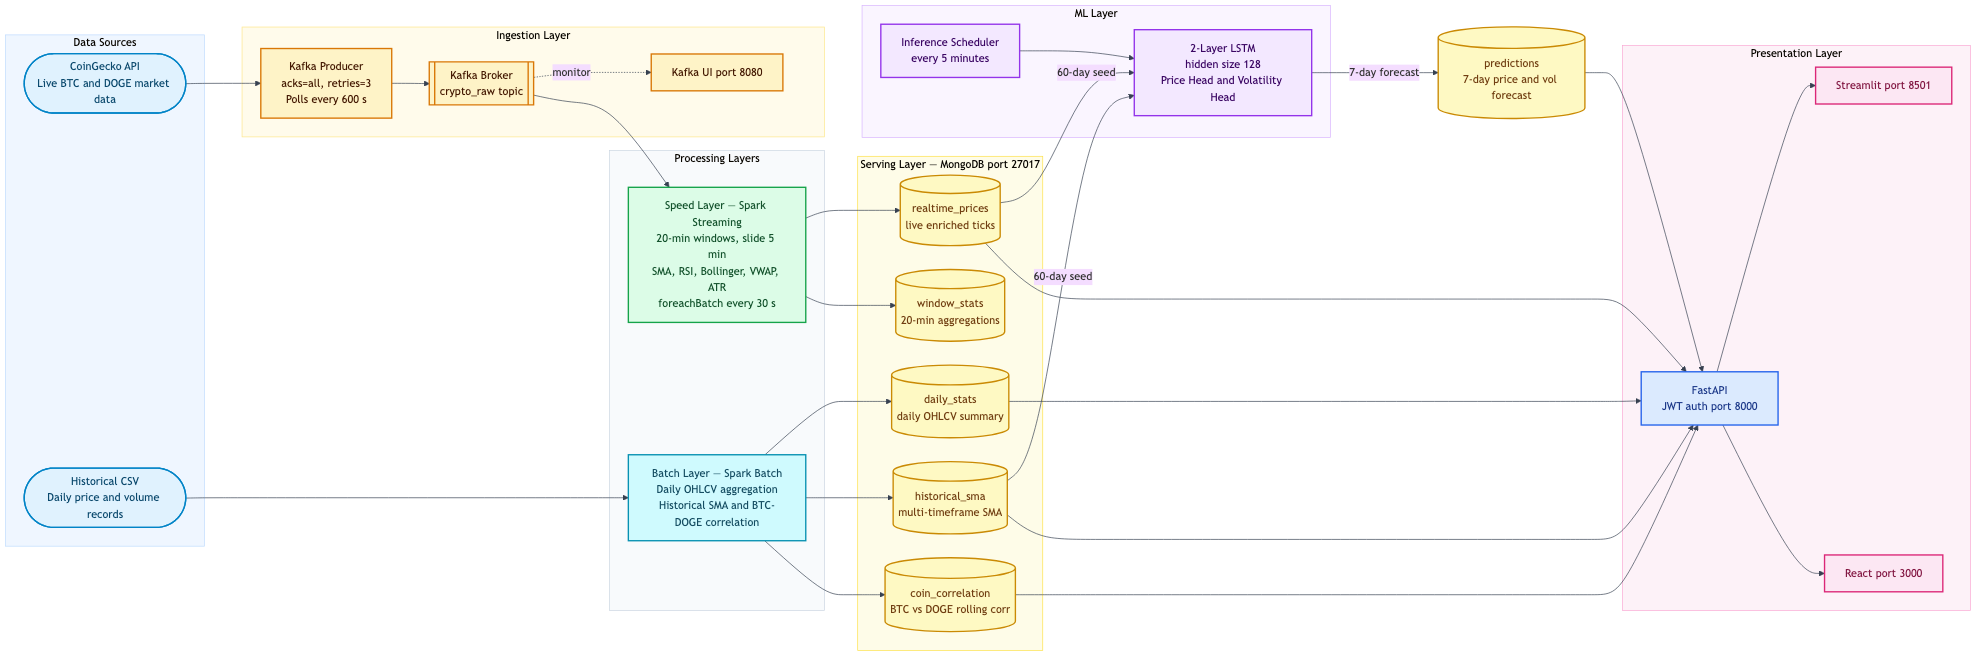
\includegraphics[width=\textwidth]{figures/architecture_overview.png}
  \caption{Sơ đồ tổng quan hệ thống: toàn bộ luồng từ nguồn dữ liệu CoinGecko đến
           các giao diện người dùng. Màu xanh dương: Batch Layer; màu xanh lá: Speed
           Layer; màu tím: Serving Layer; màu đỏ: ML Pipeline.}
  \label{fig:arch_overview}
\end{figure}

\subsection{C4 Container Model}

\begin{figure}[H]
  \centering
  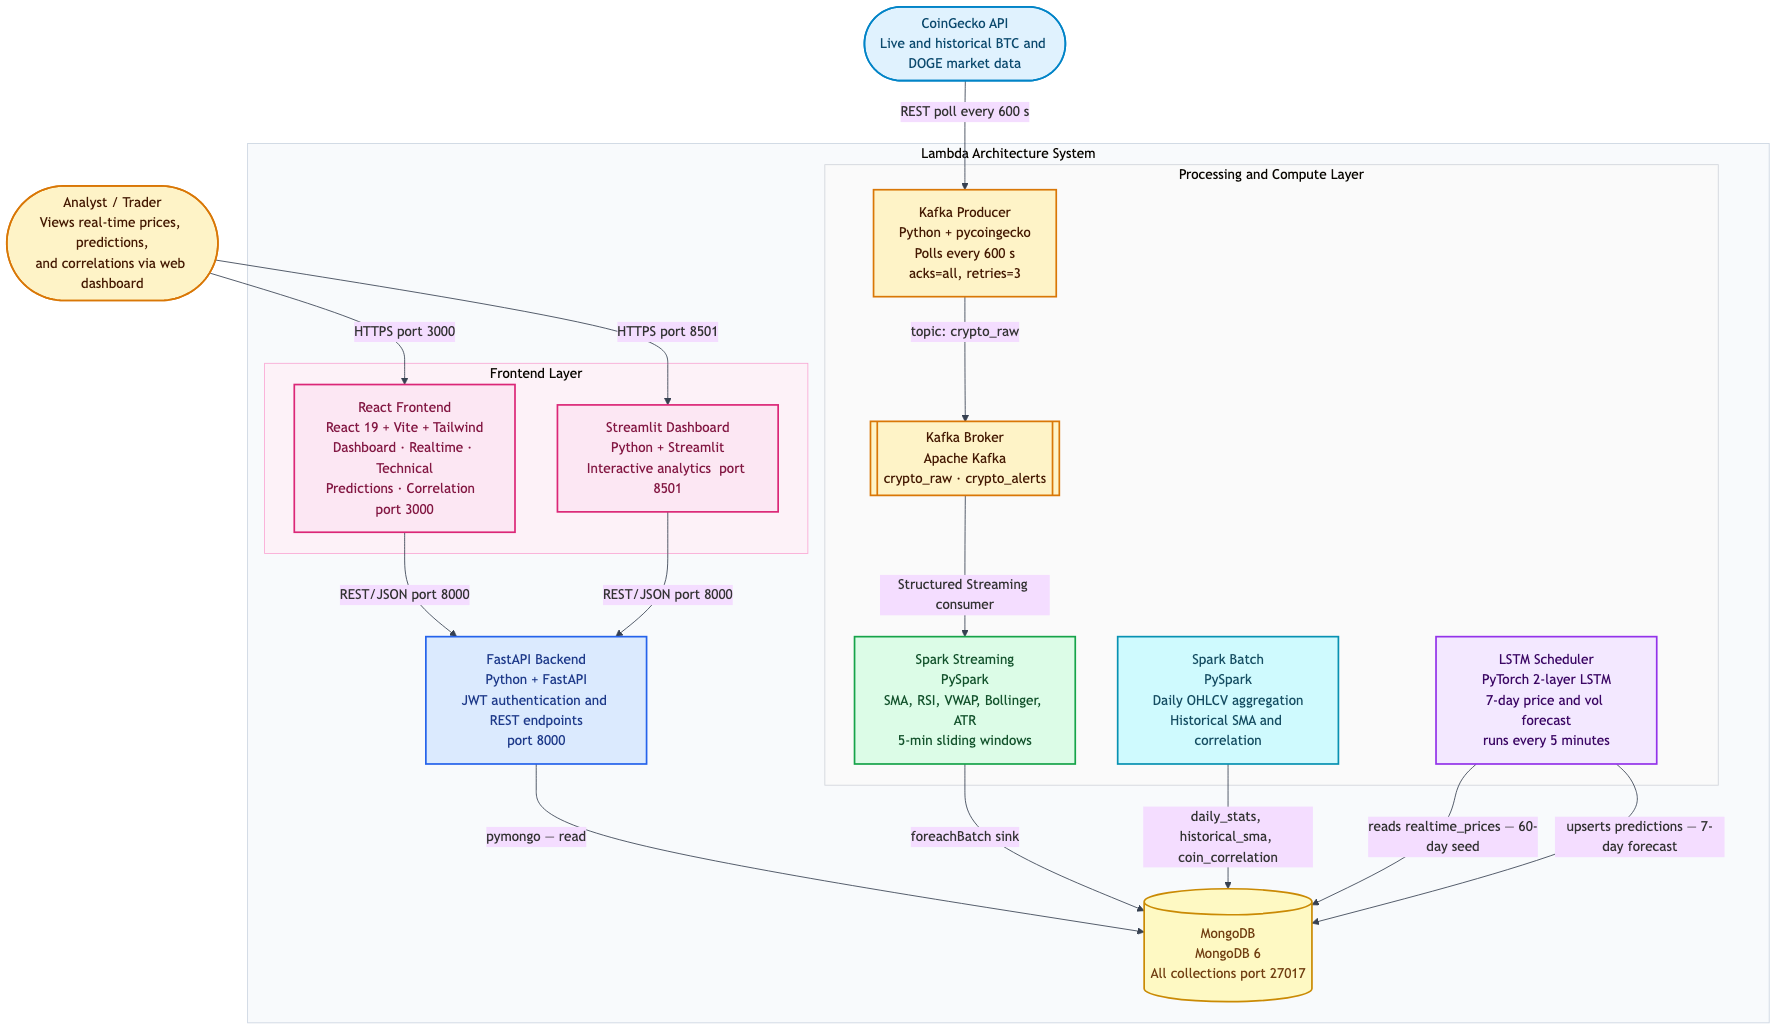
\includegraphics[width=\textwidth]{figures/architecture_c4_container.png}
  \caption{C4 Container Diagram: các container chính (Kafka, Spark, MongoDB, FastAPI,
           React, Streamlit) và luồng tương tác. Mỗi container có tên, công nghệ
           sử dụng, và mô tả trách nhiệm ngắn gọn.}
  \label{fig:c4_container}
\end{figure}

Hình~\ref{fig:c4_container} mô tả hệ thống theo mô hình C4 ở cấp Container: mỗi khối
biểu diễn một đơn vị triển khai độc lập (Docker container). Các mũi tên thể hiện
hướng phụ thuộc và giao tiếp giữa các container. Điểm đáng chú ý là MongoDB đóng
vai trò trung tâm kết nối Batch Layer, Speed Layer, ML Pipeline, và tất cả các
client --- đây là quyết định thiết kế chủ ý để giữ serving layer đơn giản và thống nhất.

\subsection{Luồng dữ liệu end-to-end}

\begin{figure}[H]
  \centering
  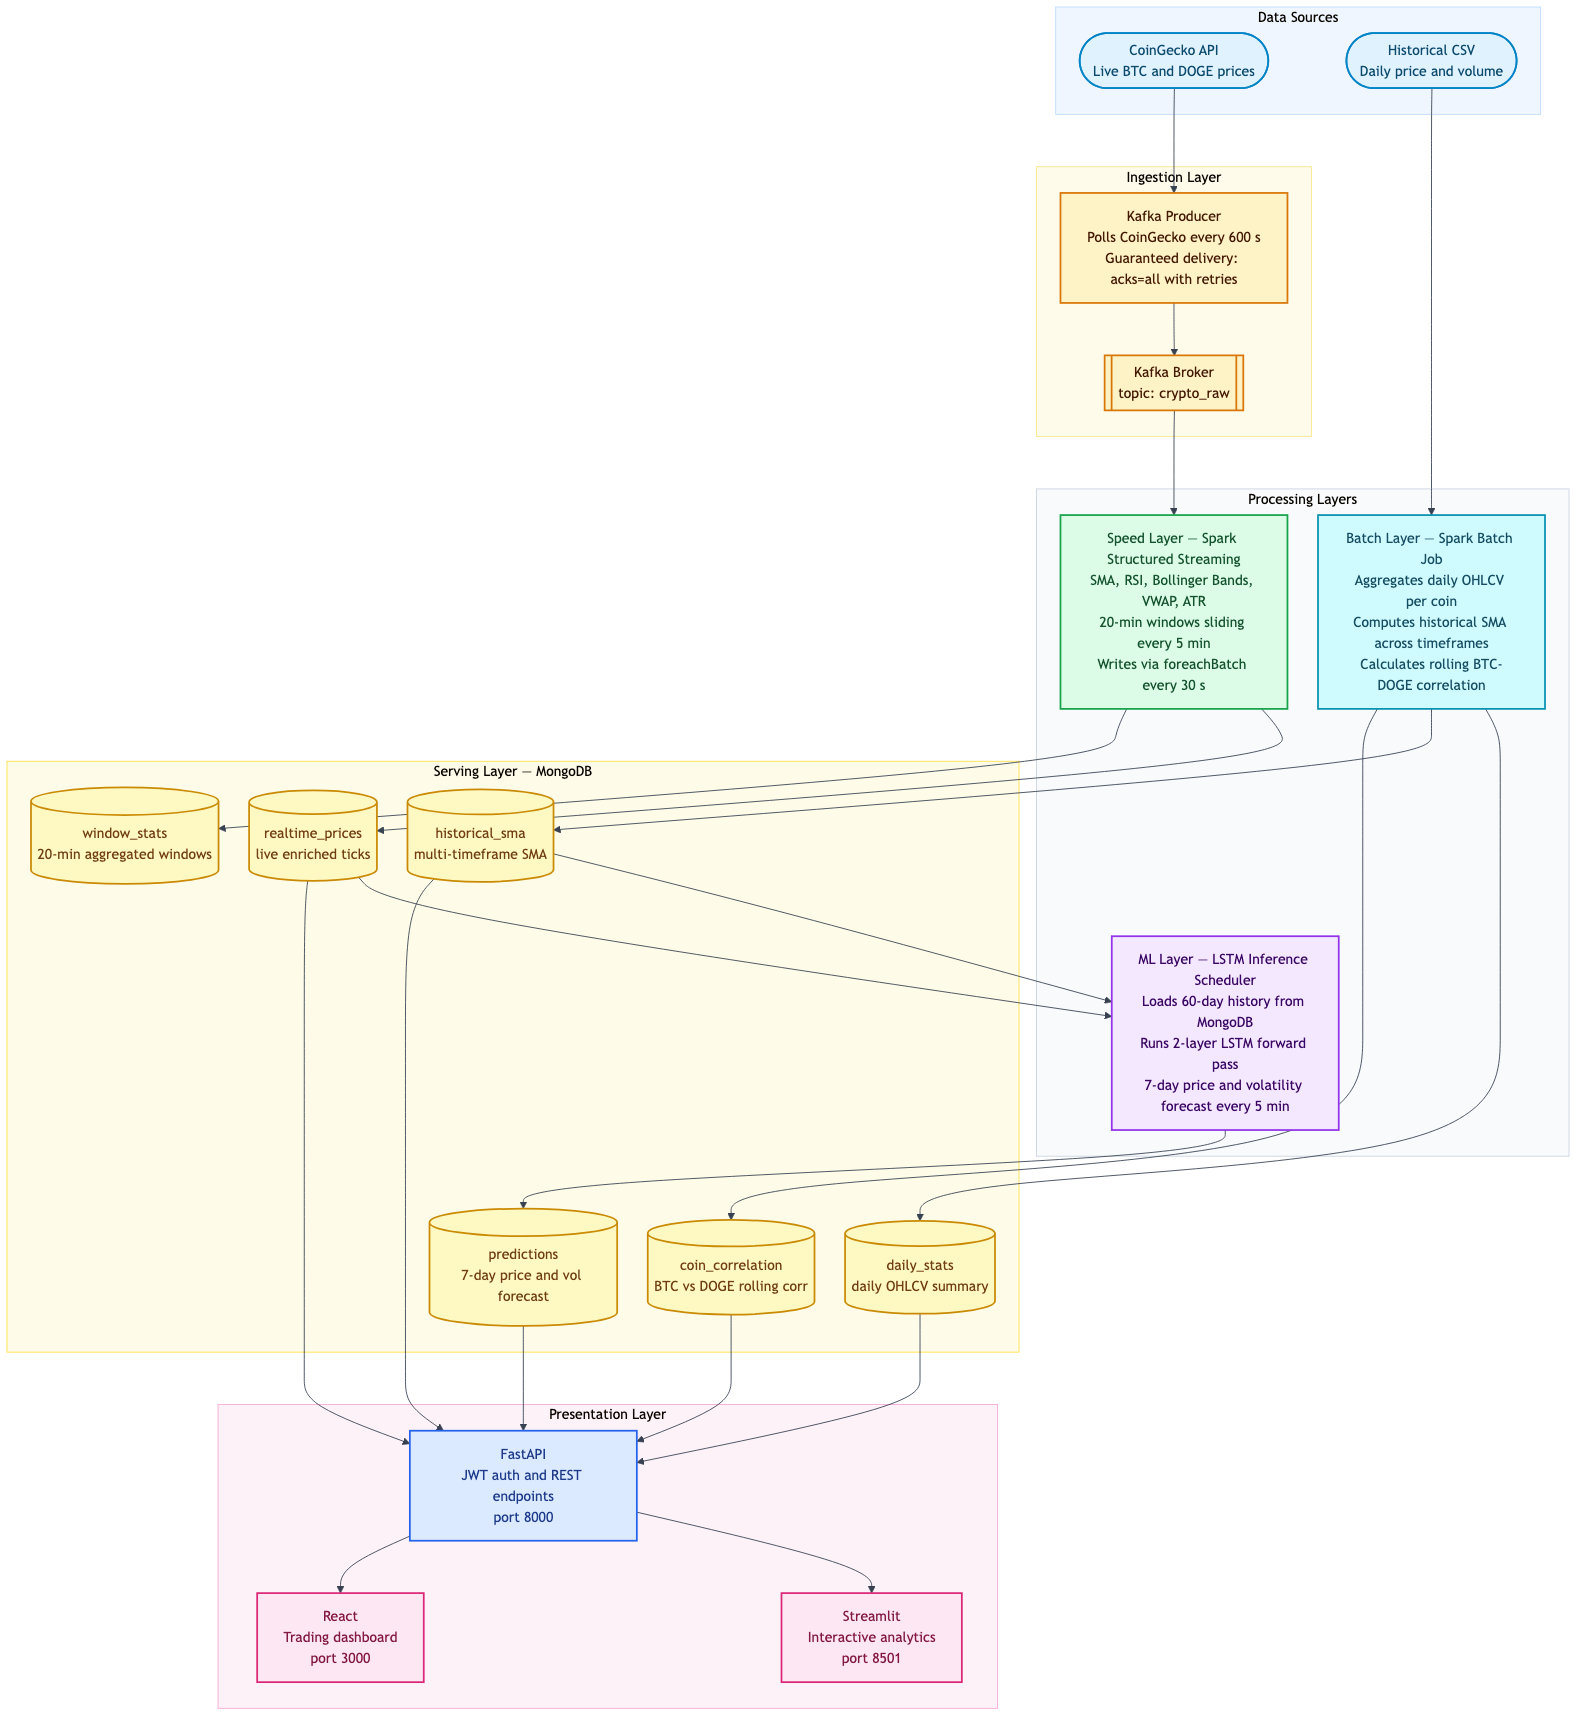
\includegraphics[width=\textwidth]{figures/architecture_dataflow.png}
  \caption{Sơ đồ luồng dữ liệu từ nguồn CoinGecko API đến sink cuối là React/Streamlit
           dashboard. Màu xanh lá: Speed Path; màu xanh dương: Batch Path; màu đỏ:
           ML Path. Mũi tên thể hiện hướng dữ liệu di chuyển.}
  \label{fig:dataflow}
\end{figure}

Có ba đường dẫn dữ liệu song song trong hệ thống (Hình~\ref{fig:dataflow}):

\begin{enumerate}
  \item \textbf{Speed Path:} CoinGecko API $\to$ Kafka Producer $\to$ topic
    \texttt{crypto\_raw} $\to$ Spark Structured Streaming $\to$ MongoDB
    (\texttt{realtime\_prices}, \texttt{window\_stats}).

  \item \textbf{Batch Path:} CSV lịch sử / MongoDB $\to$ Spark Batch Job $\to$
    MongoDB (\texttt{daily\_stats}, \texttt{historical\_sma}, \texttt{coin\_correlation}).

  \item \textbf{ML Path:} MongoDB / CSV $\to$ Feature Engineering $\to$ LSTM Training
    $\to$ Inference $\to$ MongoDB (\texttt{predictions}).
\end{enumerate}

% ============================================================
\section{Các Thành phần và Trách nhiệm}

Bảng~\ref{tab:components} tóm tắt 9 thành phần chính, công nghệ, và trách nhiệm
chức năng của từng thành phần.

\begin{table}[H]
  \centering
  \caption{Tổng quan các thành phần hệ thống và trách nhiệm}
  \label{tab:components}
  \begin{tabularx}{\textwidth}{lXX}
    \toprule
    Thành phần & Công nghệ & Trách nhiệm chính \\
    \midrule
    CoinGecko Producer & Python, pycoingecko & Thu thập giá BTC/DOGE mỗi 600 giây;
      đẩy vào Kafka với acks=all \\
    Kafka Broker & Confluent Kafka 7.4 & Hàng đợi bền vững cho dữ liệu streaming;
      đảm bảo at-least-once delivery \\
    Spark Streaming & Apache Spark 3.5 & Tính chỉ số kỹ thuật realtime (SMA, RSI,
      VWAP, Bollinger); watermark 10 phút cho late data \\
    Spark Batch & Apache Spark 3.5 & Tổng hợp daily\_stats, historical\_sma,
      coin\_correlation từ dữ liệu lịch sử \\
    MongoDB & MongoDB 6.0 & Serving layer duy nhất; lưu trữ tất cả 5 collections \\
    FastAPI Backend & Python, FastAPI & REST API với JWT authentication;
      cầu nối giữa MongoDB và clients \\
    React Frontend & React 19, TypeScript & Giao diện người dùng web; 5 trang phân
      tích với biểu đồ realtime \\
    Streamlit Dashboard & Streamlit & Dashboard phân tích nhanh cho người dùng
      nội bộ / nghiên cứu \\
    Inference Scheduler & PyTorch, schedule & Chạy LSTM inference mỗi 5 phút;
      lưu dự đoán 7 ngày vào MongoDB \\
    \bottomrule
  \end{tabularx}
\end{table}

\subsection{CoinGecko Producer}

Producer là điểm đầu vào duy nhất của dữ liệu thị trường vào hệ thống. Nó thực hiện
hai việc: (1)~gọi CoinGecko API để lấy giá tức thời và dữ liệu OHLC 4 giờ, và
(2)~serialize thành JSON và publish lên Kafka topic \texttt{crypto\_raw}.

Thiết kế đảm bảo độ tin cậy thông qua cấu hình \texttt{acks=all} (đợi tất cả ISR
replicas xác nhận) và \texttt{retries=3}. Polling interval mặc định 600 giây phù hợp
với giới hạn 10.000 lượt gọi/tháng của CoinGecko demo tier.

Mỗi message Kafka chứa đầy đủ các trường: giá (USD), market cap, khối lượng 24 giờ,
biến động 24 giờ, OHLC 4 giờ, và timestamp sự kiện.

\subsection{Speed Layer: Kafka + Spark Structured Streaming}

\begin{figure}[H]
  \centering
  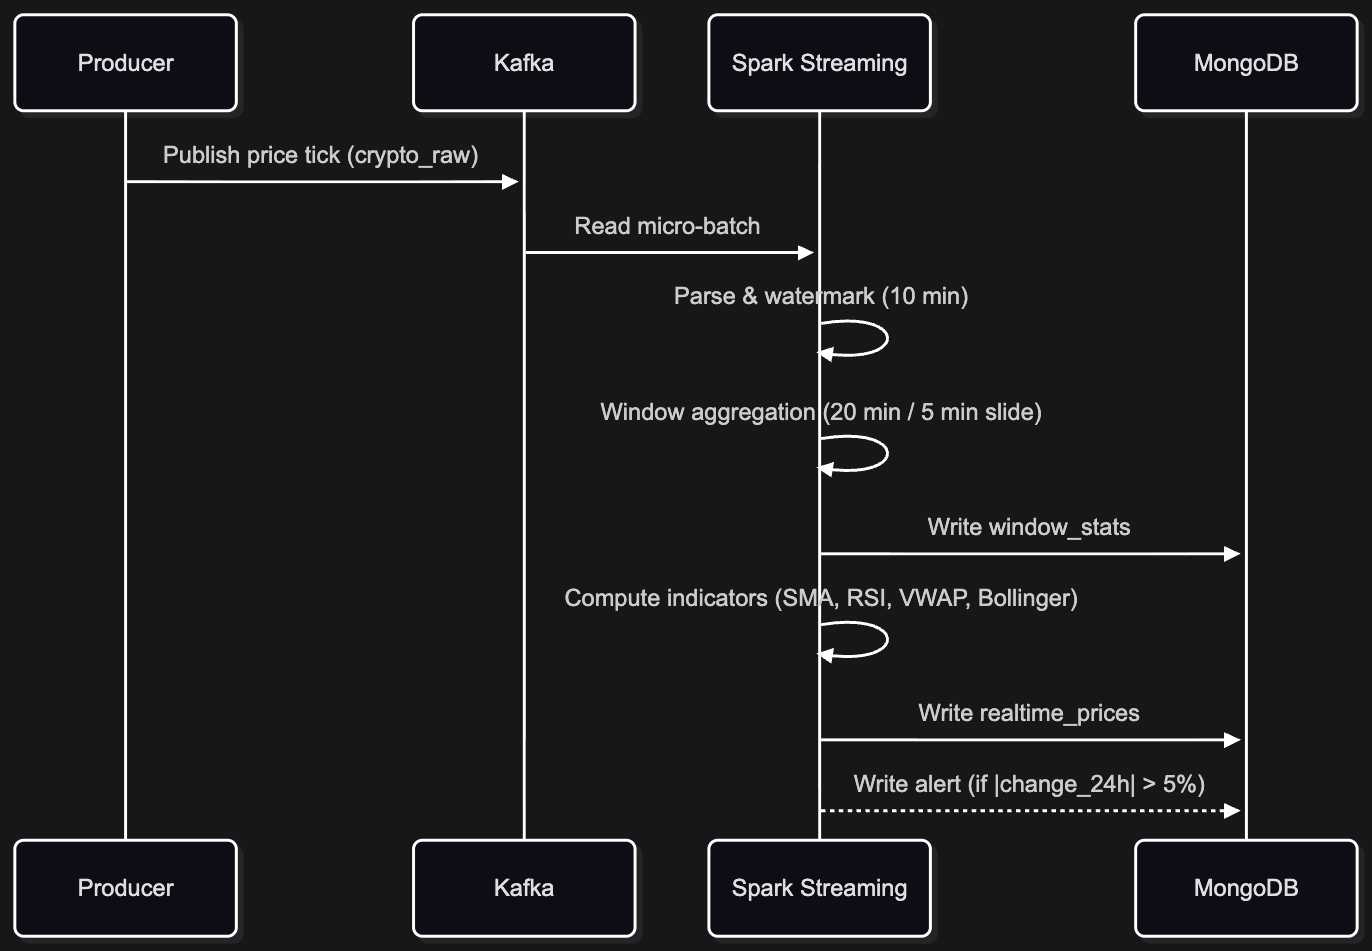
\includegraphics[width=\textwidth]{figures/diagram_spark_streaming.png}
  \caption{Luồng xử lý của Spark Structured Streaming: từ Kafka micro-batch qua
           parse và watermark, đến window aggregation và indicator computation,
           cuối cùng ghi vào MongoDB.}
  \label{fig:spark_streaming_diag}
\end{figure}

Speed Layer (Hình~\ref{fig:spark_streaming_diag}) có trách nhiệm biến đổi raw price
tick thành dữ liệu có giá trị phân tích. Luồng xử lý gồm bốn bước:

\begin{enumerate}
  \item \textbf{Đọc và parse:} Spark đọc micro-batch từ Kafka, parse JSON thành
    DataFrame có schema cố định, chuyển timestamp string thành \texttt{TimestampType}
    (UTC).

  \item \textbf{Watermark:} Áp dụng watermark 10 phút để xử lý late-arriving data
    mà không giữ state vô hạn. CoinGecko producer có thể trễ tối đa 10 phút trong
    điều kiện mạng kém.

  \item \textbf{Window aggregation (Query A):} Gom nhóm theo sliding window
    20~phút/5~phút để tính SMA-20, high, low, total volume. Kết quả ghi vào
    collection \texttt{window\_stats}.

  \item \textbf{Per-record enrichment (Query B):} Tính 5 chỉ số kỹ thuật trên
    từng record bằng PySpark Window Functions: SMA-5, SMA-20, RSI-14, VWAP-60,
    Bollinger Bands (20, 2$\sigma$). Kết quả ghi vào \texttt{realtime\_prices}.
    Nếu \texttt{|change\_24h| > 5\%}, tạo PRICE\_SPIKE alert vào MongoDB và
    Kafka topic \texttt{crypto\_alerts}.
\end{enumerate}

Cả hai query sử dụng \textbf{foreachBatch} pattern để ghi vào MongoDB thay vì
MongoDB Spark Connector, vì connector có vấn đề checkpointing trong streaming mode.
Pattern này đảm bảo exactly-once semantics thông qua delete-then-insert với batch ID.

\subsection{Batch Layer: Spark Batch Job}

Batch Layer xử lý toàn bộ dữ liệu lịch sử (4.000+ ngày) và tính toán ba tập hợp
dữ liệu mà Speed Layer không thể cung cấp do thiếu context dài hạn:

\begin{itemize}
  \item \textbf{daily\_stats:} Thống kê ngày (OHLCV, trung bình, độ lệch chuẩn) cho
    cả BTC và DOGE, dùng làm nguồn dữ liệu chính cho LSTM training.

  \item \textbf{historical\_sma:} SMA với nhiều window khác nhau (7, 14, 30, 90 ngày)
    trên toàn bộ chuỗi lịch sử.

  \item \textbf{coin\_correlation:} Rolling Pearson correlation 30 ngày giữa
    log-return BTC và DOGE --- dữ liệu cho trang Correlation trên React Frontend.
\end{itemize}

Batch job được submit thủ công hoặc theo lịch hàng ngày, đọc dữ liệu từ CSV
lịch sử, xử lý bằng Spark DataFrame API, và ghi vào MongoDB thông qua PyMongo.

\subsection{MongoDB Serving Layer}

MongoDB đóng vai trò \textbf{single serving store} cho toàn bộ hệ thống. Tất cả
writer (Spark Streaming, Spark Batch, Inference Scheduler) đều ghi vào MongoDB;
tất cả reader (FastAPI, Streamlit) đều đọc từ MongoDB. Thiết kế này đơn giản hóa
serving layer, tránh phải duy trì nhiều store khác nhau.

\begin{figure}[H]
  \centering
  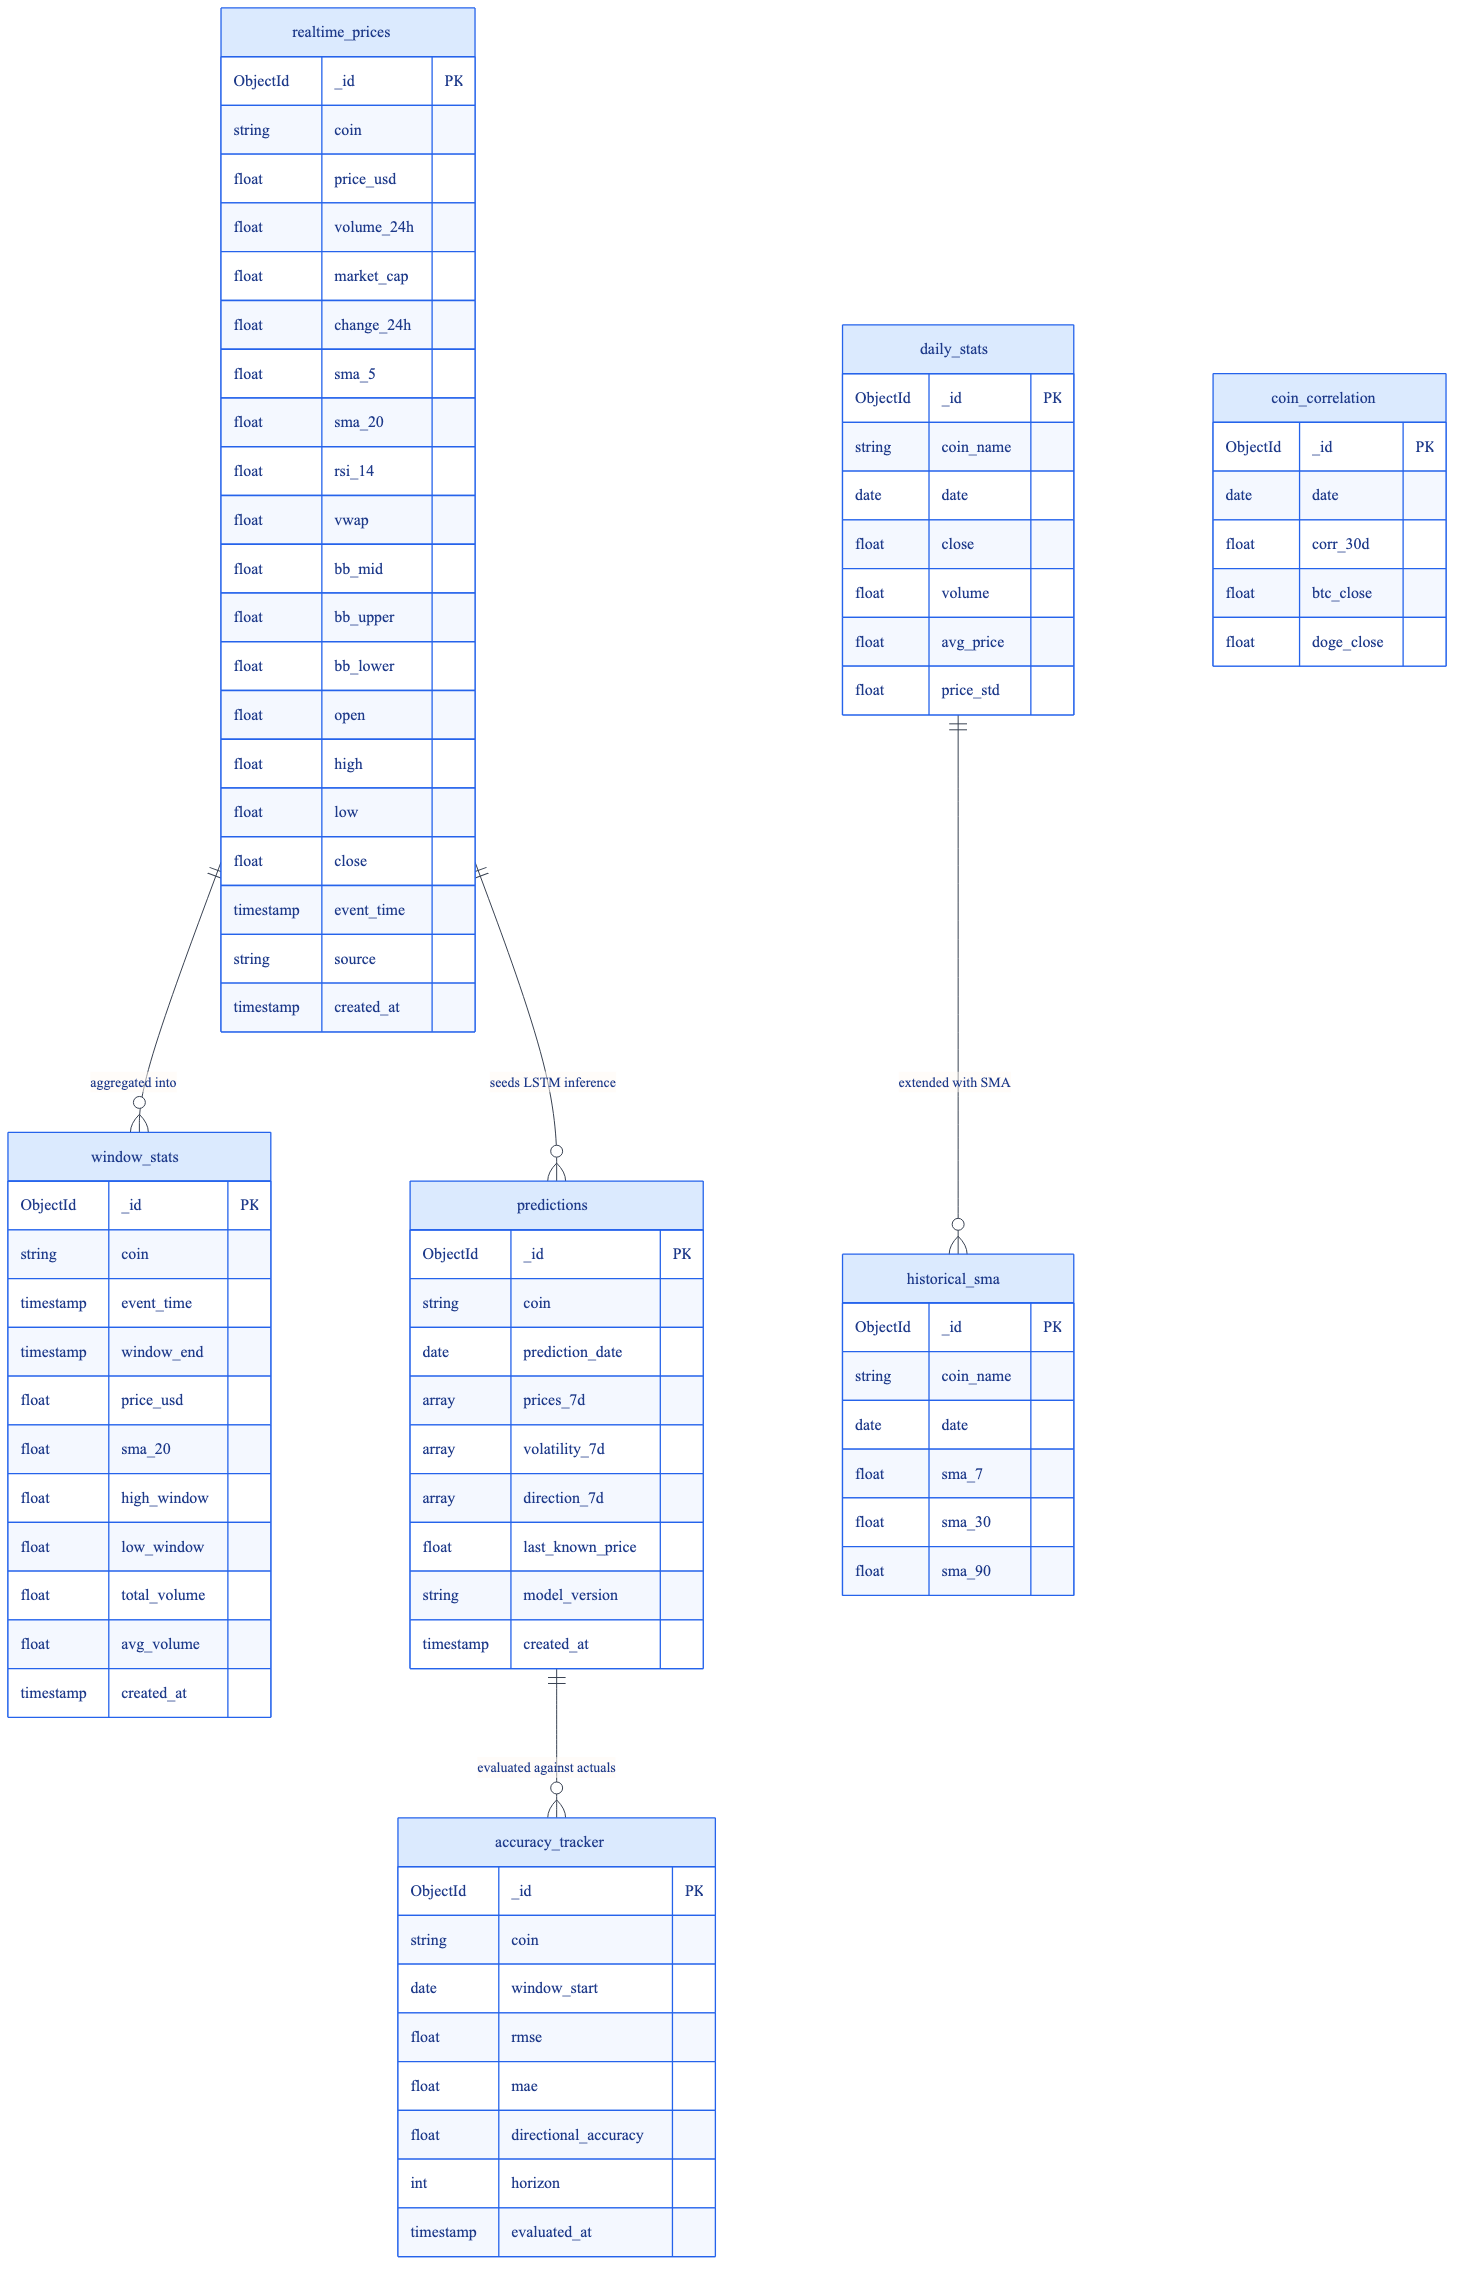
\includegraphics[width=\textwidth]{figures/diagram_mongodb_schema.png}
  \caption{Sơ đồ MongoDB schema: 5 collections với document structure, indexes, và
           TTL policies. \texttt{realtime\_prices} có TTL 7 ngày; các collection
           khác lưu trữ lâu dài với compound index trên \texttt{(coin\_name, date)}.}
  \label{fig:mongo_schema}
\end{figure}

\begin{table}[H]
  \centering
  \caption{Năm MongoDB collections và mục đích sử dụng}
  \label{tab:mongo_collections}
  \begin{tabularx}{\textwidth}{lXl}
    \toprule
    Collection & Nội dung & Writer \\
    \midrule
    \texttt{realtime\_prices} & Per-tick enriched data: OHLC + 5 chỉ số kỹ thuật
      (SMA-5, SMA-20, RSI-14, VWAP, BB). TTL 7 ngày. & Spark Streaming \\
    \texttt{window\_stats} & 20-min/5-min OHLCV rollups + SMA-20. & Spark Streaming \\
    \texttt{daily\_stats} & Daily OHLCV, avg price, std price cho BTC và DOGE. &
      Spark Batch \\
    \texttt{historical\_sma} & SMA nhiều window trên toàn bộ chuỗi lịch sử. &
      Spark Batch \\
    \texttt{coin\_correlation} & Rolling 30-ngày Pearson correlation BTC-DOGE. &
      Spark Batch \\
    \texttt{predictions} & LSTM 7-day forecast: giá dự đoán + độ biến động. &
      Inference Scheduler \\
    \texttt{alerts} & PRICE\_SPIKE events khi biến động $> 5\%$. & Spark Streaming \\
    \bottomrule
  \end{tabularx}
\end{table}

\subsection{ML Pipeline: LSTM Forecasting}

ML Pipeline hoạt động độc lập với Speed Layer và Batch Layer, đọc dữ liệu lịch sử
từ MongoDB/CSV, huấn luyện mô hình, và ghi dự đoán vào MongoDB.

\begin{figure}[H]
  \centering
  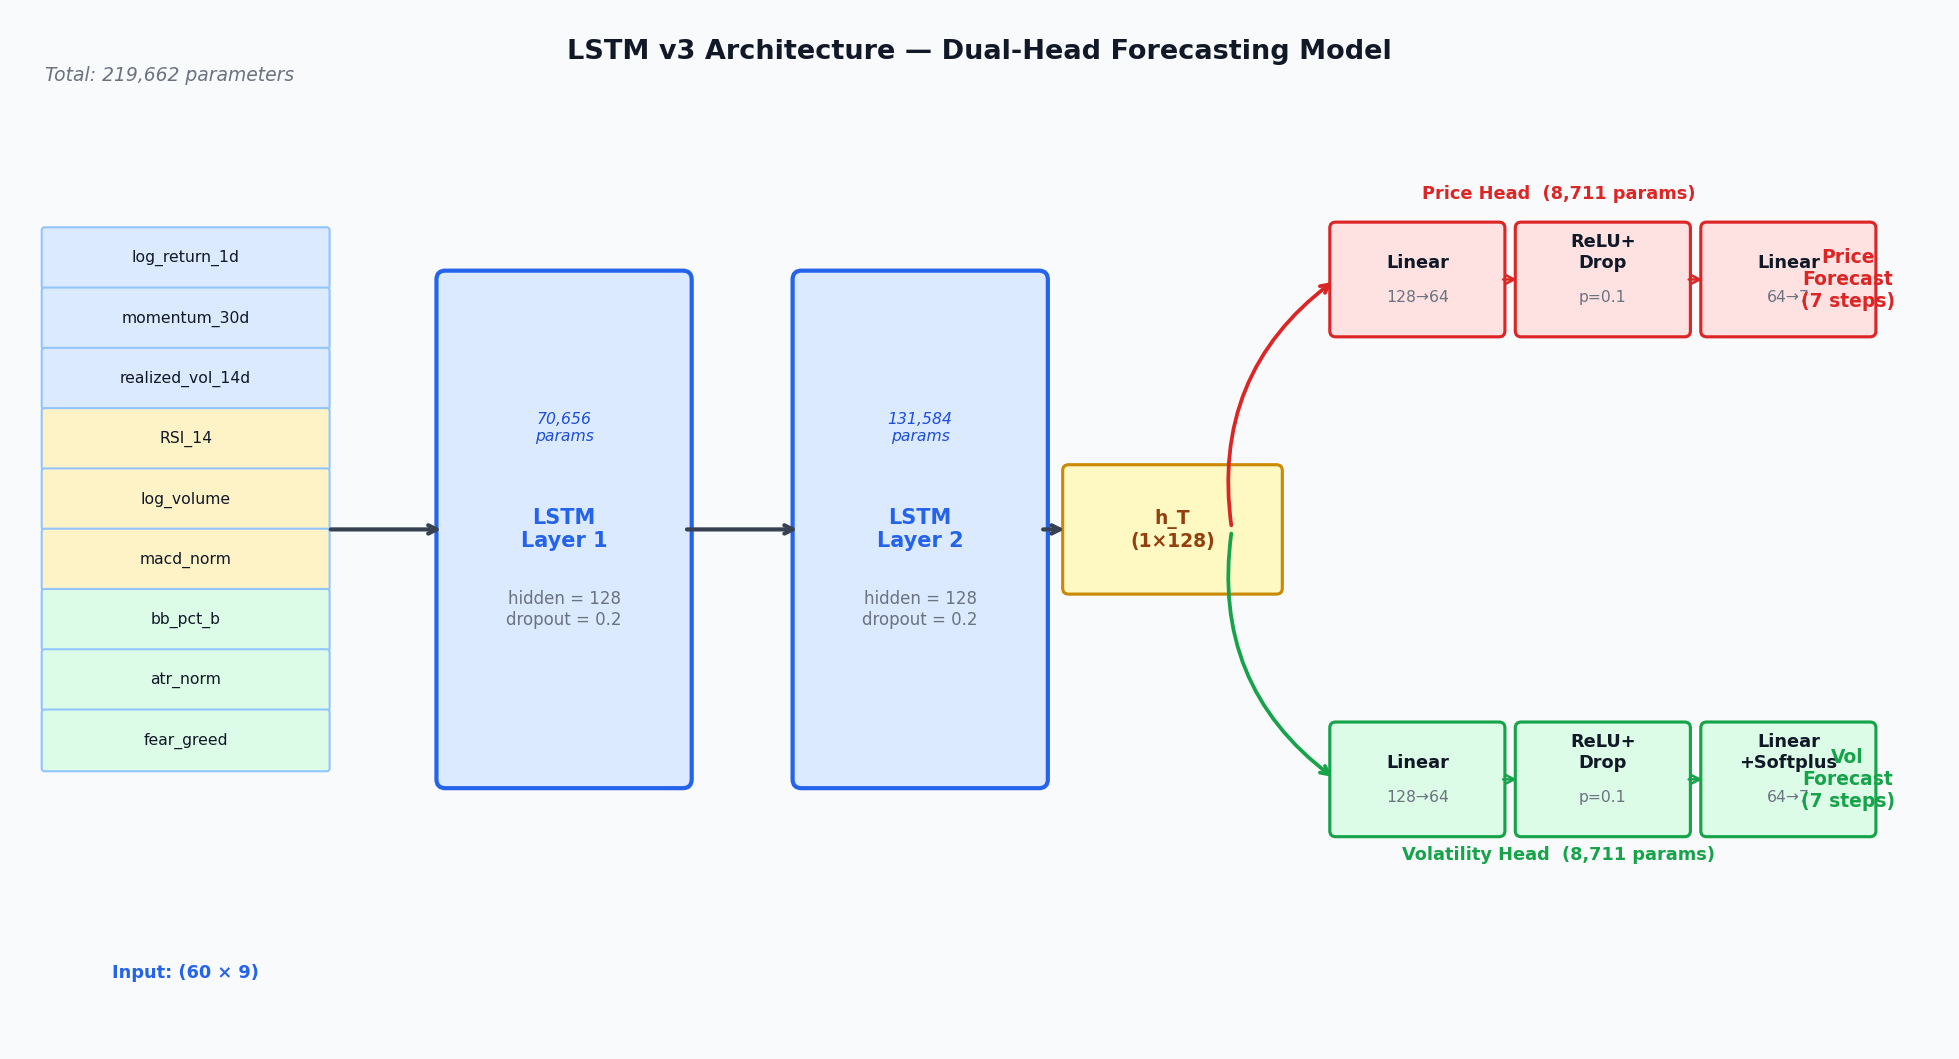
\includegraphics[width=\textwidth]{figures/lstm_architecture.png}
  \caption{Kiến trúc LSTM v3 với dual-head output: LSTM Encoder (2 lớp, 128 hidden
           units) xử lý chuỗi 60 ngày, hidden state $h_T$ được đưa vào Price Head
           (7-day forecast) và Volatility Head (confidence band) song song.}
  \label{fig:lstm_arch}
\end{figure}

\subsubsection{Feature Engineering}

Từ dữ liệu giá thô, pipeline tính 9 features chia làm 4 nhóm:

\begin{table}[H]
  \centering
  \caption{9 features đầu vào của LSTM và ý nghĩa}
  \label{tab:features}
  \begin{tabularx}{\textwidth}{llX}
    \toprule
    Feature & Nhóm & Ý nghĩa \\
    \midrule
    \texttt{log\_return\_1d} & Momentum & Tính dừng, cộng dồn được; là input
      cốt lõi cho mọi mô hình tài chính \\
    \texttt{momentum\_30d} & Momentum & Khoảng cách tương đối của giá so với SMA-30;
      nắm bắt xu hướng trung hạn \\
    \texttt{realized\_vol\_14d} & Volatility & Biến động thực tế 14 ngày; input
      chính cho Volatility Head \\
    \texttt{rsi\_14} & Oscillator & Chỉ số sức mạnh tương đối, vùng overbought/oversold \\
    \texttt{log\_volume} & Volume & Log-transform giảm skewness; volume xác nhận breakout \\
    \texttt{macd\_norm} & Oscillator & MACD chuẩn hóa theo giá; tín hiệu momentum \\
    \texttt{bb\_pct\_b} & Oscillator & Vị trí giá trong Bollinger Band (\%B) \\
    \texttt{atr\_norm} & Volatility & Proxy ATR (biên độ tức thì); bổ sung cho
      realized\_vol\_14d \\
    \texttt{fear\_greed} & Sentiment & Placeholder (= 0.5 constant); cần tích hợp
      Alternative.me API trong tương lai \\
    \bottomrule
  \end{tabularx}
\end{table}

\subsubsection{Kiến trúc Mô hình}

Mô hình LSTM v3 có ba thành phần chính:

\begin{itemize}
  \item \textbf{LSTM Encoder:} 2 lớp stacked, mỗi lớp 128 hidden units, dropout 0.2.
    Nhận chuỗi 60 timestep $\times$ 9 features. Trả về hidden state cuối $h_T \in
    \mathbb{R}^{128}$ đã encode đầy đủ ngữ cảnh 60 ngày.

  \item \textbf{Price Head:} Hai lớp fully-connected (128 $\to$ 64 $\to$ 7). Dự đoán
    7 log-return tương lai (MIMO --- Multiple Input Multiple Output). Được tái tạo
    thành giá tuyệt đối bằng cumsum.

  \item \textbf{Volatility Head:} Tương tự Price Head nhưng dùng Softplus activation
    để đảm bảo output $> 0$. Dự đoán 7 giá trị biến động tương lai, được dùng làm
    confidence interval width trên biểu đồ.
\end{itemize}

\subsubsection{Huấn luyện và Đánh giá}

\begin{figure}[H]
  \centering
  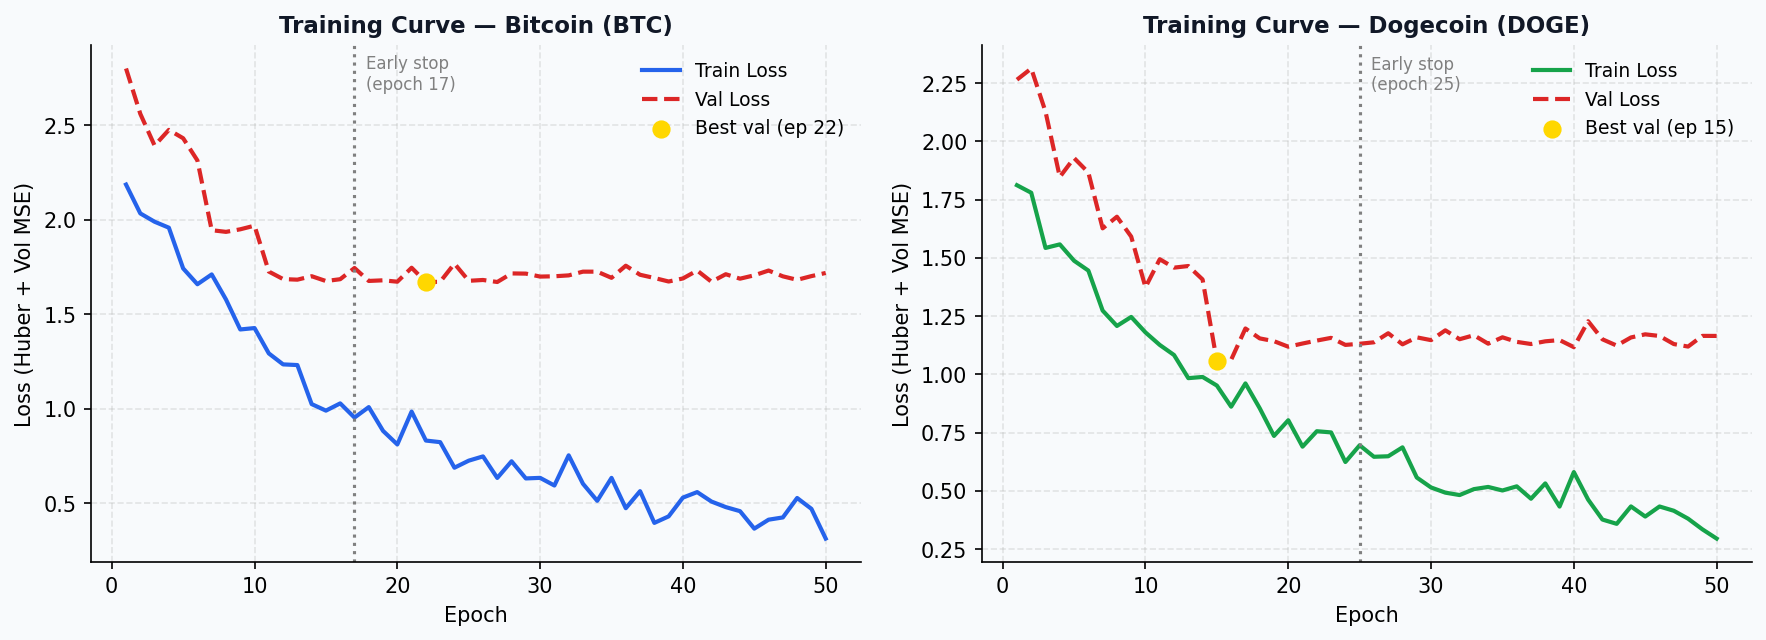
\includegraphics[width=0.9\textwidth]{figures/training_loss_curves.png}
  \caption{Đường cong loss trong quá trình huấn luyện BTC (trái) và DOGE (phải).
           Điểm vàng: best validation checkpoint. Val loss tăng sau best checkpoint
           là dấu hiệu overfitting --- được kiểm soát bởi early stopping (patience=7).}
  \label{fig:loss_curves}
\end{figure}

Quá trình huấn luyện sử dụng \textbf{direction-weighted Huber loss} kết hợp với MSE
loss cho volatility head (trọng số $\gamma = 0.3$). Direction weighting tăng penalty
gấp 3 khi mô hình dự đoán sai chiều --- phù hợp với yêu cầu thực tiễn của nhà đầu
tư quan tâm đến chiều xu hướng hơn là độ chính xác giá tuyệt đối.

\subsection{FastAPI Backend}

\begin{figure}[H]
  \centering
  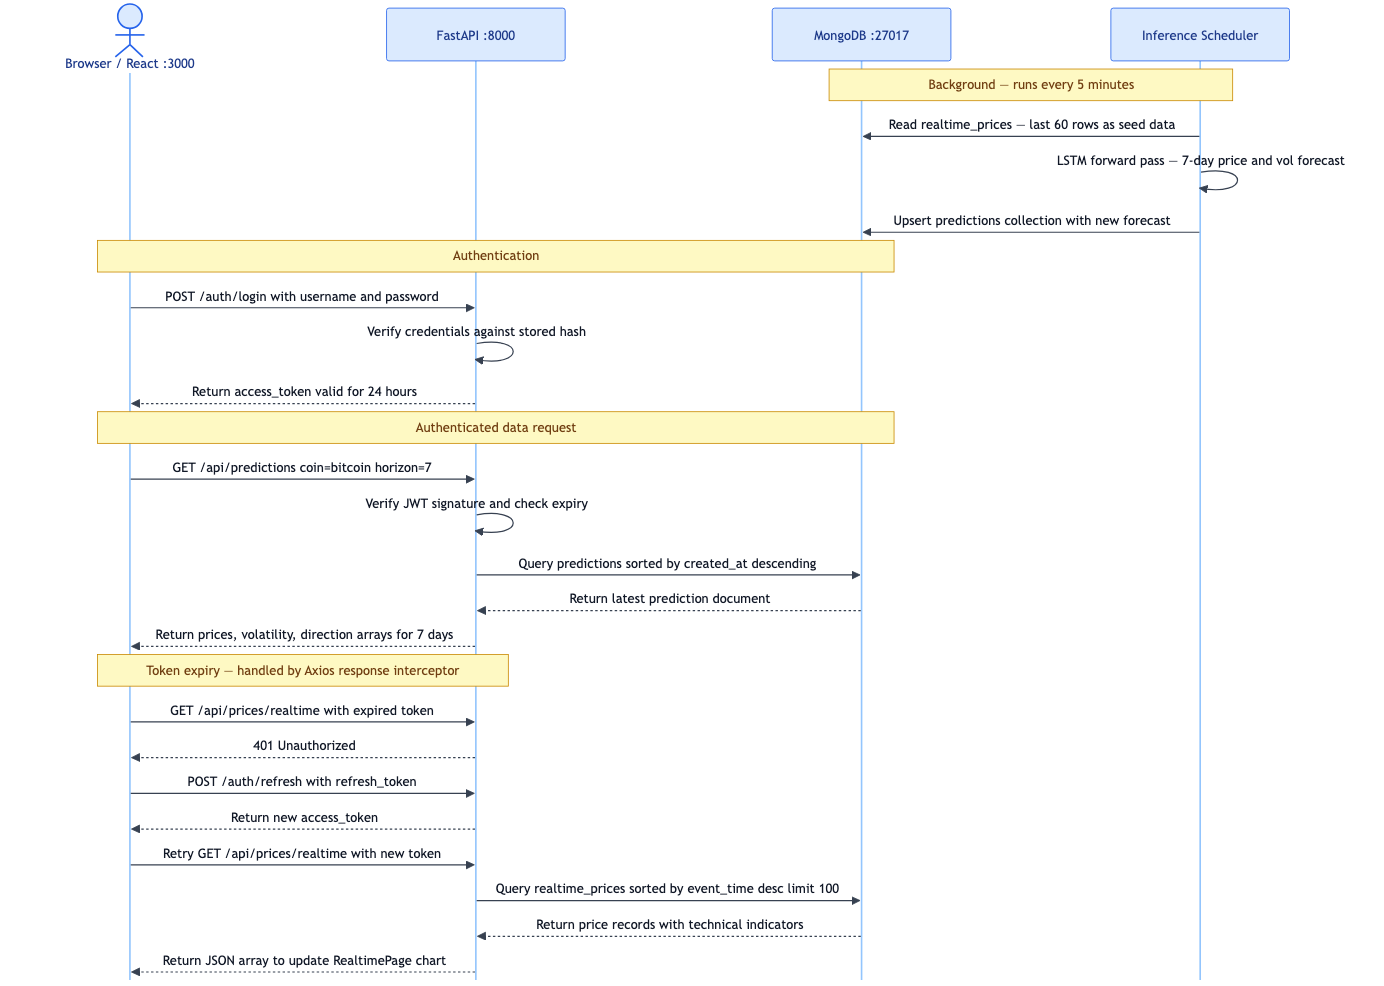
\includegraphics[width=\textwidth]{figures/diagram_api_sequence.png}
  \caption{Sequence diagram cho luồng request API điển hình: từ React client qua
           JWT middleware, đến MongoDB query, và trả về JSON response.}
  \label{fig:api_sequence}
\end{figure}

FastAPI backend là lớp giao tiếp duy nhất giữa MongoDB và các client. Thiết kế
REST API với JWT authentication đảm bảo stateless --- không cần shared session store
giữa các instance, dễ scale horizontally.

Các nhóm endpoint chính:

\begin{itemize}
  \item \textbf{/auth}: Đăng nhập, nhận JWT token (TTL 24 giờ), refresh token.
  \item \textbf{/api/prices}: Truy vấn realtime ticks và lịch sử giá.
  \item \textbf{/api/indicators}: Truy vấn chỉ số kỹ thuật (RSI, MACD, Bollinger).
  \item \textbf{/api/correlation}: Dữ liệu tương quan BTC-DOGE theo window.
  \item \textbf{/api/predictions}: Lấy dự đoán LSTM 7 ngày và accuracy tracking.
  \item \textbf{/api/models}: Model registry --- danh sách phiên bản, metrics.
\end{itemize}

\subsection{Presentation Layer: React Frontend và Streamlit}

React Frontend (React 19 + TypeScript + Vite + Tailwind CSS) cung cấp giao diện
chính cho người dùng cuối với 5 trang phân tích:

\begin{itemize}
  \item \textbf{Dashboard:} Tổng quan giá BTC/DOGE, market summary, quick stats.
  \item \textbf{Realtime:} Live price feed streaming, biểu đồ cập nhật liên tục.
  \item \textbf{Technical Analysis:} Candlestick + RSI/MACD/Bollinger overlay.
  \item \textbf{Predictions:} 7-day LSTM forecast với confidence band từ Volatility Head.
  \item \textbf{Correlation:} Rolling BTC-DOGE correlation heatmap và scatter plot.
\end{itemize}

Streamlit Dashboard phục vụ nhu cầu phân tích nhanh và trực quan hóa nội bộ, đặc
biệt hữu ích trong giai đoạn phát triển và debug.

\subsection{Inference Scheduler}

Inference Scheduler chạy liên tục như một background service, thực hiện hai nhiệm vụ
theo chu kỳ 5 phút: (1)~load mô hình LSTM đã train từ disk, chạy inference trên
60 ngày dữ liệu gần nhất, upsert 7 dự đoán vào MongoDB; (2)~so sánh các dự đoán
cũ với giá thực tế để cập nhật accuracy tracker --- dữ liệu được hiển thị trên
trang Predictions của React Frontend.

% ============================================================
\section{Triển khai Hệ thống}

\begin{figure}[H]
  \centering
  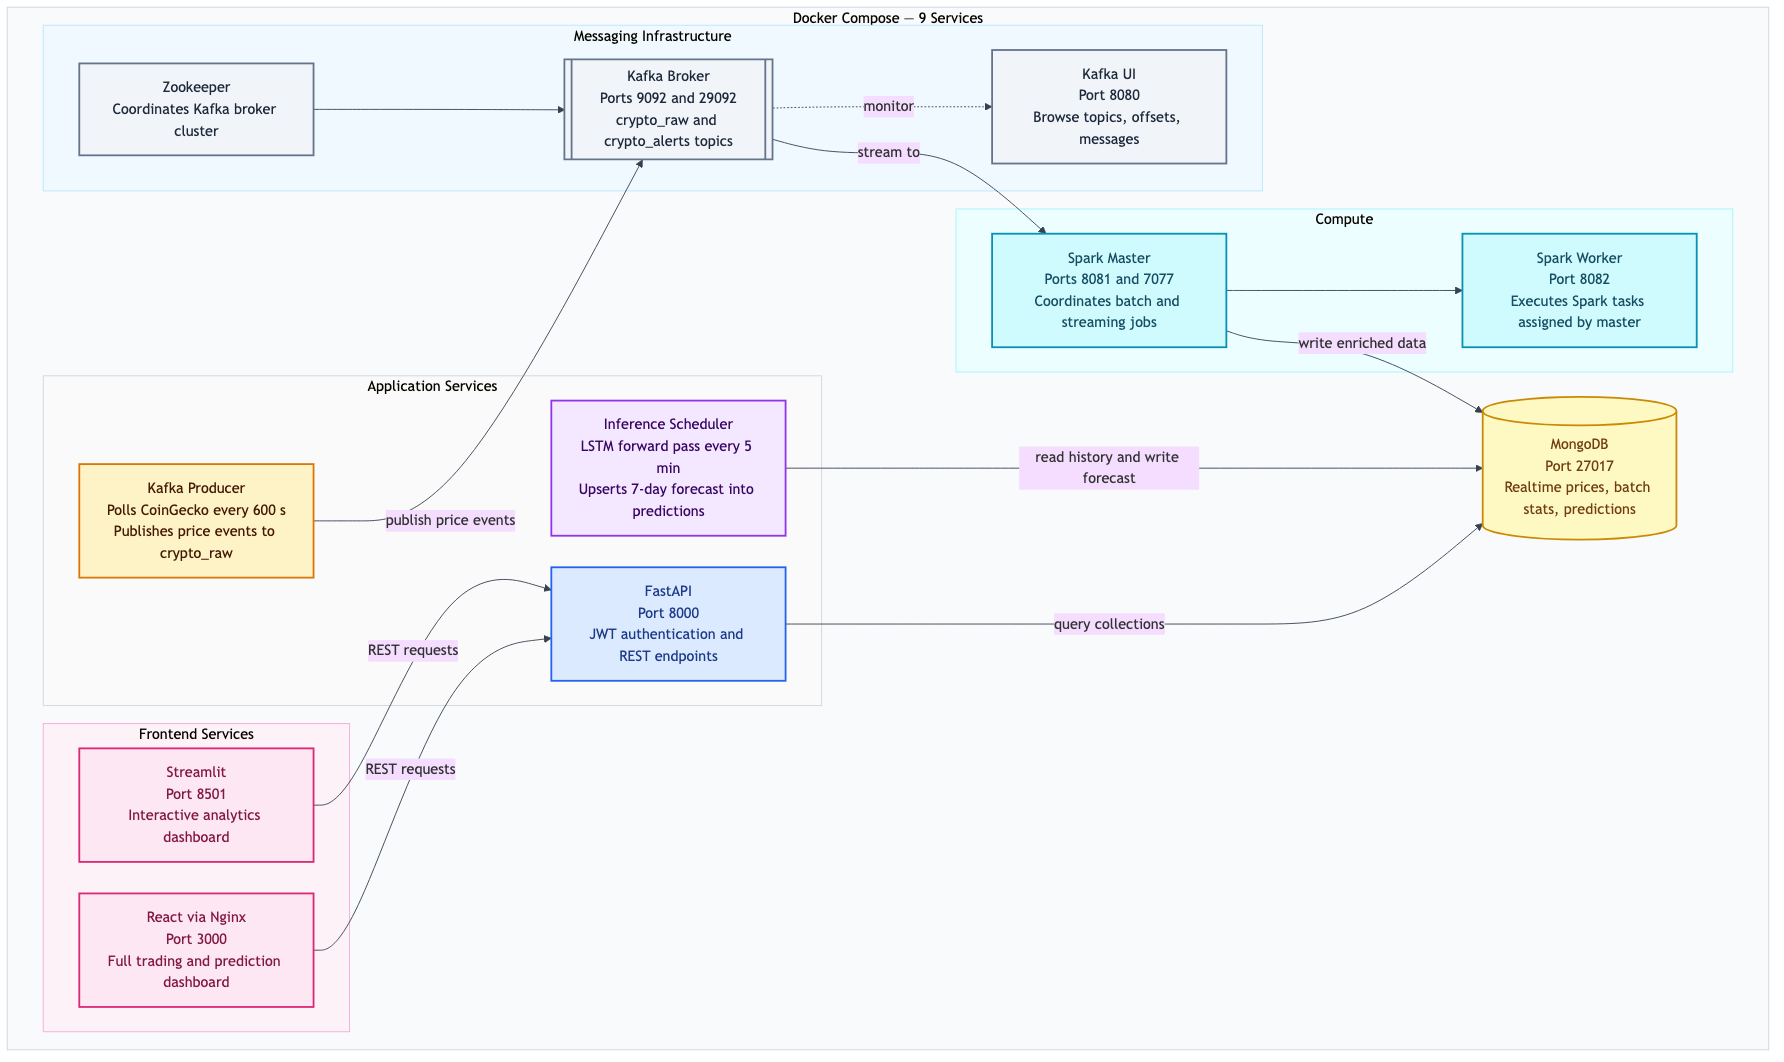
\includegraphics[width=\textwidth]{figures/architecture_deployment.png}
  \caption{Sơ đồ triển khai Docker Compose: 9 containers với network topology,
           port mapping, và volume mounts. Kafka/Zookeeper trong network riêng;
           MongoDB với persistent volume; Nginx reverse proxy cho React frontend.}
  \label{fig:arch_deployment}
\end{figure}

Toàn bộ hệ thống được đóng gói trong Docker Compose với 9 service.
Bảng~\ref{tab:docker_services} mô tả chi tiết từng service, image, port, và
dependency.

\begin{table}[H]
  \centering
  \caption{Chín Docker services, dependencies, và port}
  \label{tab:docker_services}
  \begin{tabularx}{\textwidth}{lXll}
    \toprule
    Service & Image / Role & Port & Depends On \\
    \midrule
    zookeeper & Kafka coordination & 2181 & --- \\
    kafka & Message broker & 9092 & zookeeper \\
    kafka-ui & Web UI cho Kafka & 8080 & kafka \\
    mongodb & Serving store & 27017 & --- \\
    spark-master & Spark cluster master & 8081, 7077 & --- \\
    spark-worker & Spark executor & 8082 & spark-master \\
    producer & CoinGecko ingestion & --- & kafka \\
    dashboard & Streamlit analytics & 8501 & mongodb \\
    api & FastAPI REST backend & 8000 & mongodb \\
    frontend & React + Nginx & 3000 & api \\
    inference & LSTM scheduler & --- & mongodb \\
    \bottomrule
  \end{tabularx}
\end{table}

Mỗi service có \textbf{health check} được cấu hình trong \texttt{docker-compose.yml},
đảm bảo các service phụ thuộc chỉ khởi động sau khi service mà chúng phụ thuộc đã
sẵn sàng (condition: \texttt{service\_healthy}). Điều này ngăn race condition trong
quá trình khởi động hệ thống.

% ============================================================
\section{Đảm bảo Chất lượng: Kiểm thử E2E}

\subsection{Chiến lược Kiểm thử}

Hệ thống kiểm thử được tổ chức thành hai cấp:

\begin{enumerate}
  \item \textbf{Unit Tests} (chạy không cần infrastructure): Kiểm tra từng component
    độc lập với mock dependencies. Bao gồm: \texttt{test\_lstm.py},
    \texttt{test\_indicators.py}, \texttt{test\_batch\_job.py},
    \texttt{test\_producer.py}, \texttt{test\_mongo\_writer.py},
    \texttt{test\_dashboard.py}, \texttt{test\_accuracy\_tracker.py}.

  \item \textbf{E2E Tests} (yêu cầu infrastructure thật): Ba test suite kiểm tra
    từng layer của Lambda Architecture end-to-end với Kafka và MongoDB container thật
    (testcontainers). Được đánh dấu \texttt{@pytest.mark.e2e} và loại khỏi
    \texttt{pytest} mặc định.
\end{enumerate}

\begin{infobox}
\textbf{Nguyên tắc thiết kế E2E tests:} Mỗi test suite kiểm tra \textit{đầu ra thực
tế} của một layer, không mock infrastructure. Kafka là Kafka thật; MongoDB là MongoDB
thật. Chỉ CoinGecko API được mock để kiểm soát input và tránh phụ thuộc vào network
ngoài.
\end{infobox}

\subsection{Layer 1: Producer $\to$ Kafka}

File: \texttt{tests/e2e/test\_producer\_kafka.py}

Test suite này xác nhận rằng CoinGecko Producer hoạt động đúng với một Kafka broker
thật (testcontainers). Năm test cases bao gồm:

\begin{table}[H]
  \centering
  \caption{E2E Layer 1 --- Producer to Kafka: test cases và assertion}
  \label{tab:e2e_layer1}
  \begin{tabularx}{\textwidth}{lX}
    \toprule
    Test Case & Assertion \\
    \midrule
    \texttt{test\_produces\_two\_messages\_per\_cycle} & Mỗi chu kỳ poll phải sinh
      đúng 2 message: 1 cho BTC, 1 cho DOGE. \\
    \texttt{test\_message\_schema\_is\_complete} & Message phải chứa đủ 12 trường
      bắt buộc (coin, price\_usd, volume\_24h, OHLC, timestamp, \ldots). \\
    \texttt{test\_only\_btc\_and\_doge\_produced} & Không có message nào cho
      coin ngoài BTC và DOGE. \\
    \texttt{test\_ohlc\_fields\_populated\_from\_candles} & Trường open/high/low/close
      được điền từ dữ liệu OHLC 4 giờ khi candle có sẵn. \\
    \texttt{test\_message\_values\_are\_correct} & Giá trị trong message khớp với
      dữ liệu mock CoinGecko (kiểm tra end-to-end correctness). \\
    \bottomrule
  \end{tabularx}
\end{table}

\begin{infobox}
\textbf{Tại sao test này quan trọng?} Đây là điểm đầu vào duy nhất của dữ liệu vào
hệ thống. Nếu schema message sai, toàn bộ pipeline downstream sẽ thất bại. Test suite
này đảm bảo contract giữa Producer và Consumer (Spark Streaming) luôn được giữ.
\end{infobox}

\subsection{Layer 2: Spark Batch $\to$ MongoDB}

File: \texttt{tests/e2e/test\_batch\_mongo.py}

Test suite này xác nhận rằng Spark Batch Job tạo ra đúng các aggregation và ghi vào
MongoDB với schema và giá trị hợp lệ. Được tổ chức thành 3 class theo collection:

\begin{table}[H]
  \centering
  \caption{E2E Layer 2 --- Spark Batch to MongoDB: test cases và assertion}
  \label{tab:e2e_layer2}
  \begin{tabularx}{\textwidth}{llX}
    \toprule
    Class & Test Case & Assertion \\
    \midrule
    \multirow{4}{*}{TestDailyStats}
      & \texttt{test\_row\_count\_positive} & Collection không được rỗng sau batch job. \\
      & \texttt{test\_only\_btc\_and\_doge} & Chỉ có BTC và DOGE, không có coin khác. \\
      & \texttt{test\_required\_columns} & Có đủ các cột: date, close, volume, avg\_price, price\_std. \\
      & \texttt{test\_prices\_are\_positive} & Mọi giá trị close và volume đều $> 0$. \\
    \midrule
    \multirow{3}{*}{TestHistoricalSma}
      & \texttt{test\_row\_count\_matches} & Số row SMA khớp với số row daily\_stats. \\
      & \texttt{test\_has\_sma\_columns} & Có đủ cột SMA-7, SMA-14, SMA-30, SMA-90. \\
      & \texttt{test\_only\_btc\_and\_doge} & Scope coin đúng. \\
    \midrule
    \multirow{4}{*}{TestCoinCorrelation}
      & \texttt{test\_exactly\_one\_pair} & Chỉ có một pair BTC-DOGE. \\
      & \texttt{test\_pair\_is\_btc\_doge} & Tên coins trong document đúng. \\
      & \texttt{test\_pearson\_value\_in\_range} & Giá trị correlation $\in [-1, 1]$. \\
      & \texttt{test\_no\_ethereum} & Không có Ethereum trong bảng correlation. \\
    \bottomrule
  \end{tabularx}
\end{table}

\subsection{Layer 3: ML Pipeline $\to$ MongoDB}

File: \texttt{tests/e2e/test\_ml\_mongo.py}

Test suite này xác nhận toàn bộ ML pipeline: từ training, lưu model artifact, đến
inference và ghi dự đoán vào MongoDB. Hai class chính:

\begin{table}[H]
  \centering
  \footnotesize
  \caption{E2E Layer 3 --- ML Pipeline to MongoDB: test cases và assertion}
  \label{tab:e2e_layer3}
  \begin{tabular}{p{7.2cm}p{6.8cm}}
    \toprule
    \textbf{Test Case} & \textbf{Assertion} \\
    \midrule
    \multicolumn{2}{l}{\textit{Class: TestLstmTraining}} \\
    \midrule
    \texttt{test\_training\_returns\_metrics}      & Training trả về dict chứa RMSE, MAE, directional accuracy. \\[3pt]
    \texttt{test\_model\_file\_saved}              & File \texttt{lstm\_\{coin\}\_v2.pt} được lưu đúng path. \\[3pt]
    \texttt{test\_scaler\_file\_saved}             & File \texttt{scaler\_\{coin\}.pkl} được lưu đúng path. \\[3pt]
    \texttt{test\_rmse\_is\_non\_negative}         & RMSE $\geq 0$. \\[3pt]
    \texttt{test\_mae\_is\_non\_negative}          & MAE $\geq 0$. \\[3pt]
    \texttt{test\_directional\_accuracy\_in\_range}& Dir.\ accuracy $\in [0, 1]$. \\
    \midrule
    \multicolumn{2}{l}{\textit{Class: TestInferenceToMongo}} \\
    \midrule
    \texttt{test\_writes\_7\_predictions}              & Inference ghi đúng 7 document vào \texttt{predictions}. \\[3pt]
    \texttt{test\_prediction\_document\_schema}        & Document có đủ trường: coin, date, predicted\_price, model\_version. \\[3pt]
    \texttt{test\_predicted\_prices\_are\_positive}    & Mọi giá dự đoán $> 0$. \\[3pt]
    \texttt{test\_prediction\_dates\_are\_in\_future}  & 7 ngày dự đoán đều sau ngày hiện tại. \\[3pt]
    \texttt{test\_prediction\_dates\_are\_unique}      & Không có ngày trùng lặp. \\[3pt]
    \texttt{test\_upsert\_idempotency}                 & Chạy inference hai lần vẫn chỉ có 7 document (upsert). \\
    \bottomrule
  \end{tabular}
\end{table}

\begin{infobox}
\textbf{Test \texttt{test\_upsert\_idempotency}:} Đây là test quan trọng nhất của Layer 3.
Inference Scheduler chạy mỗi 5 phút --- nếu không idempotent, MongoDB sẽ tích lũy hàng
nghìn documents trùng lặp. Test này đảm bảo upsert pattern hoạt động đúng và hệ thống
có thể restart mà không gây data corruption.
\end{infobox}

\subsection{Ma trận Phủ Kiểm thử}

Bảng~\ref{tab:test_coverage} thể hiện mỗi thành phần được kiểm thử ở cấp nào và
thuộc tính nào được xác nhận.

\begin{table}[H]
  \centering
  \caption{Ma trận phủ kiểm thử: thành phần và cấp kiểm thử}
  \label{tab:test_coverage}
  \begin{tabularx}{\textwidth}{lXcc}
    \toprule
    Thành phần & Thuộc tính được kiểm thử & Unit & E2E \\
    \midrule
    Producer & Schema message, giá trị, OHLC & \checkmark & \checkmark \\
    Kafka & Message delivery, consumer read & --- & \checkmark \\
    Spark Indicators & SMA, RSI, VWAP, Bollinger correctness & \checkmark & --- \\
    Spark Batch & Row count, schema, coin scope, value range & \checkmark & \checkmark \\
    MongoDB Writer & Upsert pattern, idempotency & \checkmark & \checkmark \\
    LSTM Model & Forward pass shape, loss computation & \checkmark & --- \\
    LSTM Training & Artifact save, metrics range & --- & \checkmark \\
    Inference & 7-day output, positive prices, upsert idempotency & --- & \checkmark \\
    Accuracy Tracker & Comparison logic, metric calculation & \checkmark & --- \\
    Dashboard & Widget render, data loading & \checkmark & --- \\
    \bottomrule
  \end{tabularx}
\end{table}

% ============================================================
\section{Đánh giá Mô hình LSTM}

\subsection{Walk-Forward Validation}

\begin{figure}[H]
  \centering
  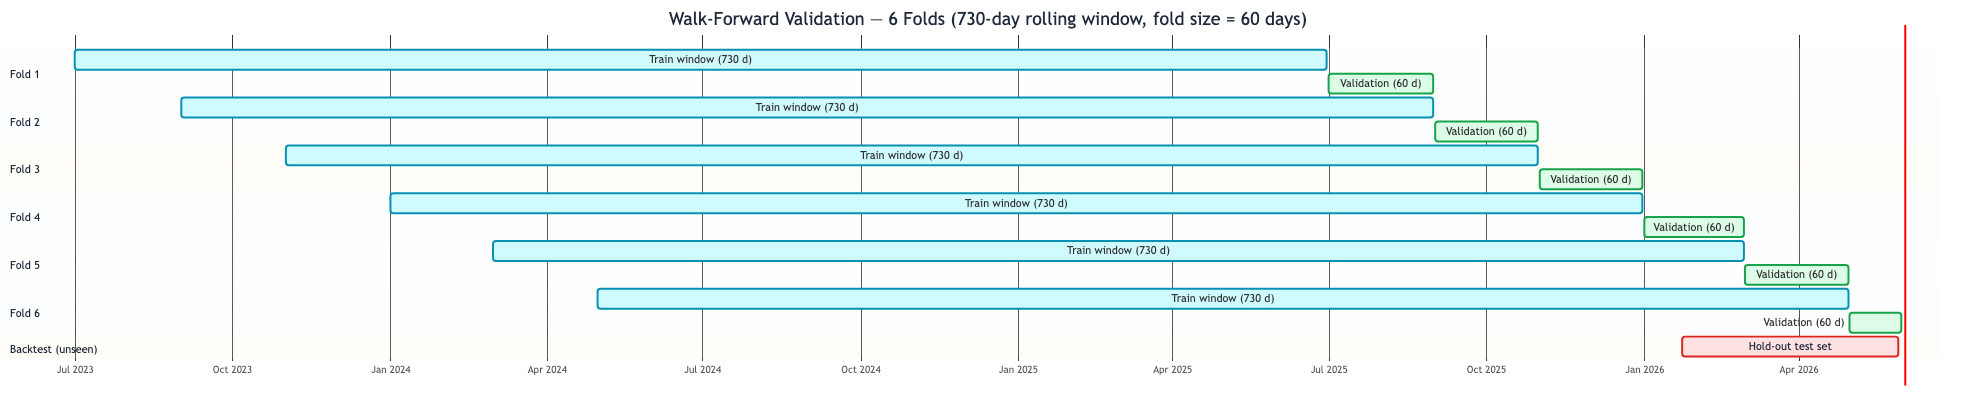
\includegraphics[width=\textwidth]{figures/diagram_walk_forward.png}
  \caption{Sơ đồ walk-forward validation với 6 folds: mỗi fold mở rộng training
           window theo thời gian (rolling 730 ngày), validation window 60 ngày ngay
           sau training. Không có overlap giữa các val window.}
  \label{fig:wf_diag}
\end{figure}

Walk-forward validation được chọn thay vì K-Fold vì K-Fold shuffle dữ liệu ngẫu nhiên,
gây temporal leakage --- mô hình train trên dữ liệu tương lai rồi test trên quá khứ
\cite{ref9}. Walk-forward tôn trọng thứ tự thời gian: mỗi fold luôn train trên dữ liệu
trước và validate trên dữ liệu sau.

\begin{table}[H]
  \centering
  \caption{Kết quả walk-forward 6 fold --- Bitcoin ($H = 7$)}
  \label{tab:wf_detail}
  \begin{tabular}{crrrc}
    \toprule
    Fold & RMSE (\$) & MAE (\$) & Dir Acc (\%) & Ghi chú \\
    \midrule
    1 & 3.902 & 2.840 & 46,3 & Sideway market \\
    2 & 3.029 & 2.415 & 50,0 & \\
    3 & 4.810 & 3.773 & 50,0 & Sideway (post-halving) \\
    4 & 3.160 & 2.378 & \textbf{55,6} & Trending market \\
    5 & 4.144 & 2.972 & 38,9 & Sideway \\
    6 & 2.581 & 2.094 & \textbf{55,6} & Trending market \\
    \midrule
    \textbf{Mean} & \textbf{3.604} & \textbf{2.579} & \textbf{49,4} & \\
    \bottomrule
  \end{tabular}
\end{table}

Mô hình cho kết quả tốt hơn rõ rệt trên trending market (fold 4, 6: 55,6\%) so với
sideway market (fold 3, 5: 38,9--50\%). Đây là đặc tính phổ biến của mô hình chuỗi
thời gian: tín hiệu xu hướng rõ ràng hơn khi thị trường có hướng.

\subsection{Backtest 6 Tháng}

\begin{figure}[H]
  \centering
  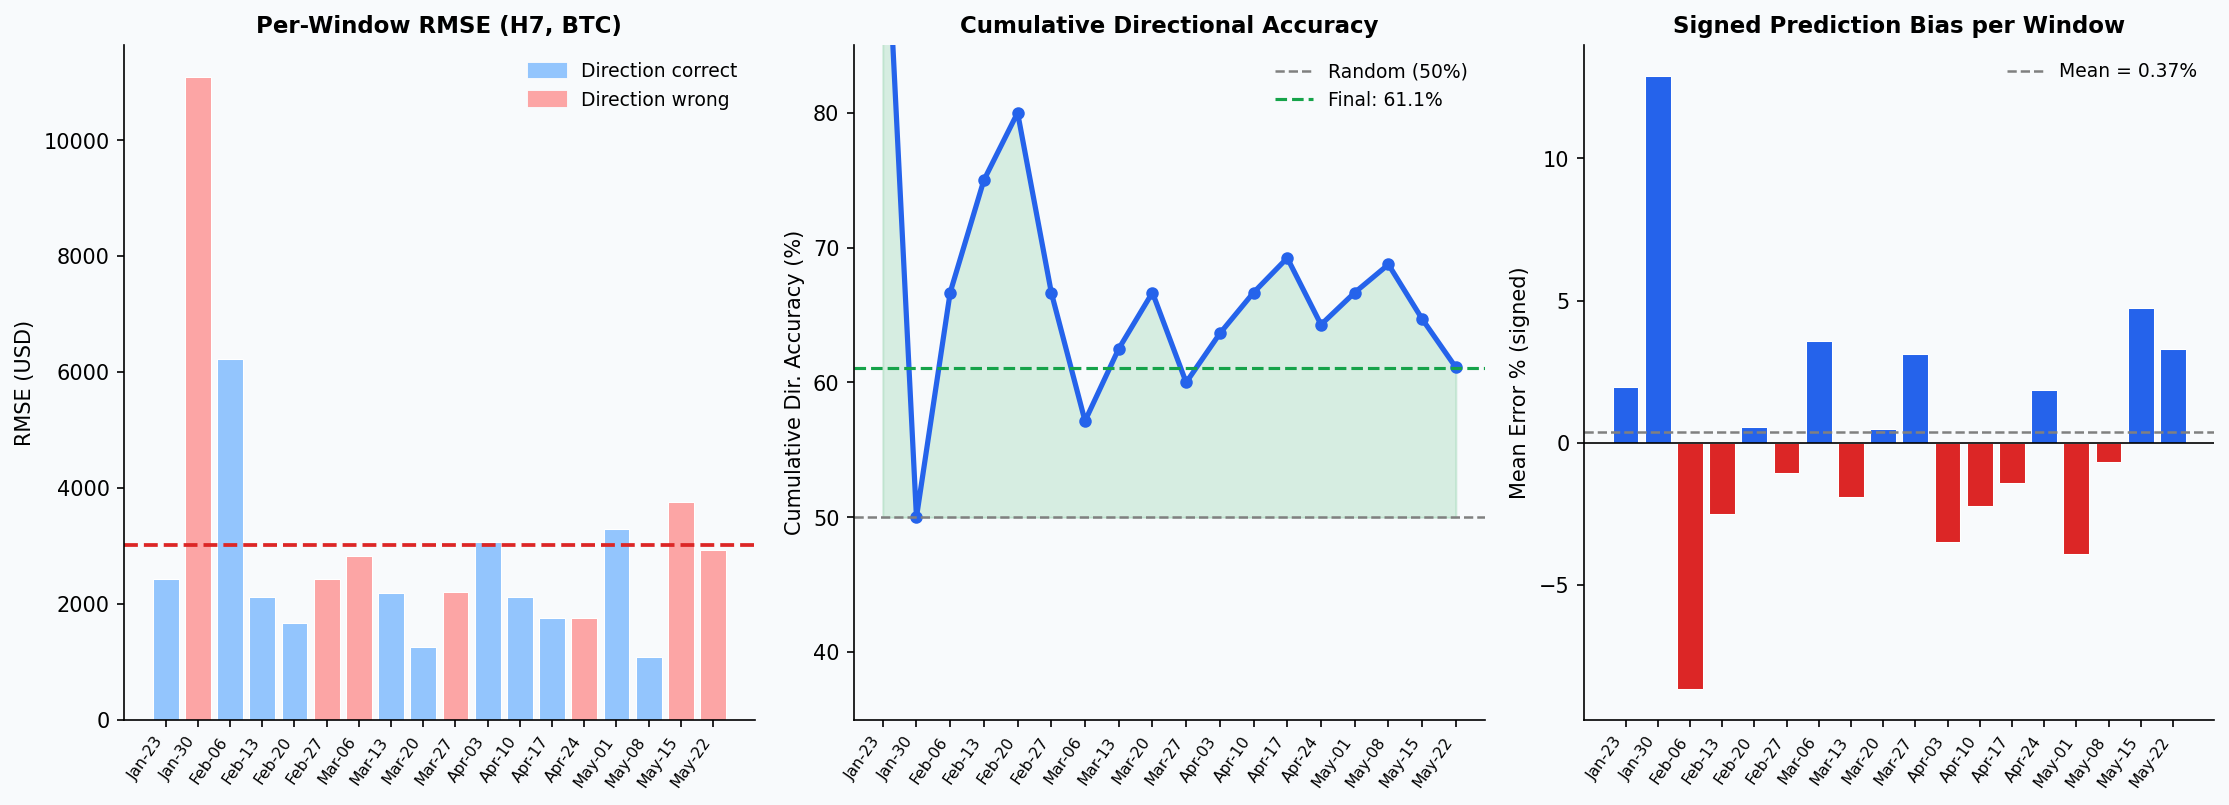
\includegraphics[width=\textwidth]{figures/backtest_analysis.png}
  \caption{Phân tích backtest 6 tháng BTC (H=7): RMSE per-window (trái), directional
           accuracy tích lũy (giữa), và signed prediction bias (phải). Directional
           accuracy ổn định trên 50\% từ cửa sổ thứ 7 trở đi.}
  \label{fig:backtest_detail}
\end{figure}

\begin{figure}[H]
  \centering
  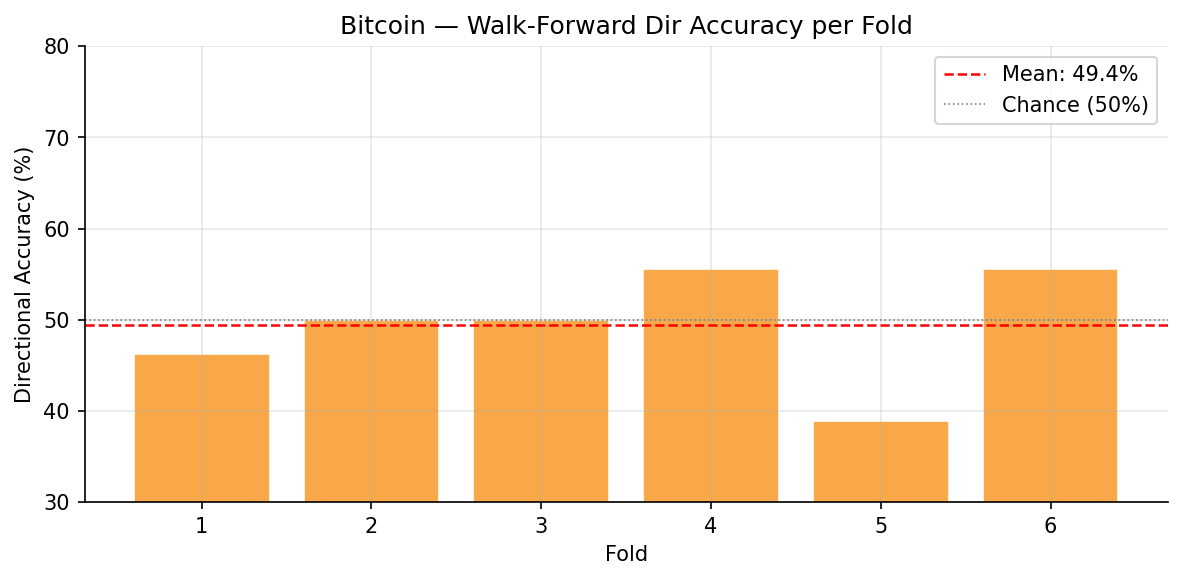
\includegraphics[width=\textwidth]{figures/walk_forward_dir_acc.png}
  \caption{Directional accuracy theo từng fold: BTC (xanh dương) và DOGE (cam).
           Đường nét đứt đỏ là ngưỡng 50\% (random baseline). DOGE nhất quán dưới
           BTC do noise-to-signal ratio cao hơn.}
  \label{fig:wf_dir_acc}
\end{figure}

\begin{table}[H]
  \centering
  \caption{Backtest BTC theo ba horizon (01/2026 -- 05/2026)}
  \label{tab:backtest_multi}
  \begin{tabular}{lrrrr}
    \toprule
    Horizon & Windows & RMSE trung bình & Dir Acc & Nhận xét \\
    \midrule
    7 ngày  & 18 & \$3.010 & \textbf{61,1\%} & Practical signal \\
    15 ngày & 8  & \$4.290 & 50,0\%          & Random \\
    60 ngày & 2  & \$13.453 & 50,0\%         & Unreliable \\
    \bottomrule
  \end{tabular}
\end{table}

\begin{infobox}
\textbf{Kết quả quan trọng:} H7 đạt 61,1\% directional accuracy trên 18 cửa sổ test
thực tế --- vượt ngưỡng random 11,1 điểm phần trăm. Horizon ngắn (7 ngày) là vùng
hữu ích duy nhất của mô hình; horizon dài hơn không có tín hiệu đáng tin cậy.
\end{infobox}

\begin{warnbox}
\textbf{Giới hạn:} 18 cửa sổ backtest là mẫu nhỏ. Mô hình cũng không tự retrain
khi market regime thay đổi --- Inference Scheduler chỉ chạy inference, không retrain.
Cần cơ chế weekly retrain để duy trì hiệu suất dài hạn.
\end{warnbox}

% ============================================================
\section{Giới hạn Kỹ thuật}

\begin{enumerate}
  \item \textbf{Rate limiting CoinGecko:} Demo tier giới hạn 10.000 lượt gọi/tháng.
    Producer không thể poll nhanh hơn 600 giây mà không vượt quota \cite{ref7}.

  \item \textbf{Thiếu OHLC đầy đủ:} ATR proxy dùng $|r_t|$ thay vì True Range thực
    sự. Cần nguồn dữ liệu OHLC (Binance, Kraken) để tính ATR chính xác.

  \item \textbf{fear\_greed placeholder:} Feature 8 luôn bằng 0,5, không đóng góp
    thông tin. Có thể xóa hoặc thay bằng Alternative.me API.

  \item \textbf{Single-node Spark:} Local mode không scale. Với nhiều coin hơn hoặc
    dữ liệu tick-by-tick, cần Spark cluster thực.

  \item \textbf{Không tự retrain:} Mô hình LSTM được train một lần. Khi market
    regime thay đổi, hiệu suất có thể giảm mà hệ thống không tự phát hiện.
\end{enumerate}

% ============================================================
\section{Kết luận}

Tài liệu này đã trình bày thiết kế kiến trúc hệ thống phân tích tiền mã hóa theo
ba chiều: \textit{cấu trúc} (Lambda Architecture với ba layer), \textit{thành phần}
(9 service với trách nhiệm rõ ràng), và \textit{chất lượng} (chiến lược kiểm thử
E2E ba layer).

Điểm mạnh chính của thiết kế là sự phân tách rõ ràng giữa Speed Layer (realtime
indicators), Batch Layer (historical aggregations), và ML Pipeline (predictions) ---
ba concerns này có yêu cầu khác nhau về latency, correctness, và computational cost,
và Lambda Architecture giải quyết chúng một cách độc lập.

Chiến lược kiểm thử E2E với testcontainers (Kafka thật, MongoDB thật) đảm bảo rằng
các contract giữa các component được giữ không chỉ ở cấp unit mà còn ở cấp system.
Đặc biệt, test idempotency cho ML inference và test schema contract cho Producer là
hai safety net quan trọng nhất của hệ thống.

% ============================================================
\bibliographystyle{unsrtnat}
\bibliography{references}

\end{document}
